% notes can be: hide, only or show
\documentclass[ignorenonframetext,red,8pt,notes=show]{beamer}

\usepackage[utf8]{inputenc}
\usepackage{beamerthemesplit}
\usepackage{graphics}
\usepackage{natbib}
\usepackage[english]{babel}
\usepackage{url}
\usepackage{times}
\usepackage[T1]{fontenc}
\usepackage{hyperref}
\usepackage{epstopdf}
\usepackage{subfig}

\usepackage{multirow}
\usepackage{rotating}

\usepackage{booktabs}


% hack for beamer and natbib working together
%\newcommand{\newblock}{}

\mode<presentation>
{
	\usetheme{Warsaw}
    % remove sections and subsections form each slide
    \setbeamertemplate{headline}{}
    %\setbeamertemplate{headline}{\vspace{0.05cm}}
    % center frame titles
    \setbeamertemplate{frametitle}[default][center]
    % remove navigation buttons
    \beamertemplatenavigationsymbolsempty
% 	\usecolortheme{lily}
}

\mode<article>
{
  \usepackage{fullpage}
  \usepackage{pgf}
%  \setjobnamebeamerversion{beamerexample2.beamer}
}

\usepackage{fancyvrb}
\usepackage{color}
%\usepackage{colortbl}
\usepackage{listings}
%\usepackage{listings,bera}
\definecolor{keywords}{RGB}{128,148,182}
%\definecolor{comments}{RGB}{60,179,113}
\definecolor{comments}{RGB}{0,0,139}
\lstset{language=Python,
        %numbers=false,
        showstringspaces=false,
        numberstyle=\tiny,
        %frame=leftline,
        numbersep=4.5pt,
  keywordstyle=\color{keywords}\bfseries,
  commentstyle=\color{comments}\emph
}

\hypersetup{
%   pdfpagemode=FullScreen, % Sembla que no funciona correctament
  unicode=true,
  pdftitle={The Structural Dimension of Cooperation},%
  pdfauthor={Jordi Torrents},%
  pdfcreator={},%
  pdfproducer=PDFLaTeX,%
  pdfsubject={},%
  pdfkeywords={}%
}

%\AtBeginSection[]{\frame{\frametitle{Contents}\tableofcontents[current]}}

\title{The Structural Dimension of Cooperation}
\subtitle{Cooperation Networks as Cohesive Small Worlds\\PhD Thesis Defense}
\author{Jordi Torrents}
\institute{Department of Sociology\\University of Barcelona}

\begin{document}

\begin{frame}[label=portada]
\maketitle
\end{frame}

%\begin{frame}[label=toc]
%\frametitle{Contents}
%\tableofcontents
%\end{frame}

\section{Large Scale Cooperation}

\begin{frame}
\frametitle{Large Scale Cooperation}

The last half of twentieth century has witnessed a key shift in knowledge intensive production processes.

\begin{block}{The rising importance of collective research and cooperation \citep{uzzi:2007a}}
\begin{itemize}
\item During most of the last century important papers or inventions were mostly developed by a single author 
\item Since 2000s top cited papers or inventions are developed by a team.
\end{itemize}
\end{block}

\pause

\begin{block}{\textbf{Socialization} concept drawn from the Marxian tradition \citep{adler:2007}}
\begin{itemize}
\item In Political Science: transfer of ownership from the private to the public sphere.
\item In Psychology: process whereby people new to a culture internalize its knowledge, norms and values.
\item Marx's use was broader than either and encompasses both:
\end{itemize}
\begin{quote}
The [...] socialized (i.e. collective) labour come into being through cooperation, division of labour within the workshop, the use of machinery, and in general, the transformation of production by the conscious use of the sciences, of mechanics, chemistry, etc. for specific ends, technology, etc. and similarly, through the enormous increase of scale corresponding to such developments (for it is only socialized labour that is capable of applying the general products of human development, such as mathematics, to the immediate process of production; [...]). \citep[1024]{marx:1990}
\end{quote}
\end{block}

\end{frame}
\note{\citet*{uzzi:2007a} show that until 1950s the likelihood that an important ---ie wildly cited--- paper or invention was developed by a single author was bigger than it was developed by a team. But this trend has experimented a shift in the last four decades. The rising importance of collective research and cooperation is illustrated by the fact that top cited papers are mostly created by teams in 2000s.}



\subsection{Theoretical Approaches to Cooperation}
\begin{frame}[label=]
\frametitle{Theoretical Approaches to Cooperation}

\begin{columns}[c]
\begin{column}{0.5\textwidth}

\begin{block}{Macro level approach}
Cooperation as a macro level phenomenon in which the center of analysis is the collective or group \citep{marx:1990, adler:2006, adler:2015}.

\begin{itemize}

\item Focus on large organizations and groups: Collaborative Communities

\begin{itemize}

\item Shared values and goals
\item Generalized trust
\item Authority forms

\end{itemize}
\end{itemize}
\end{block}
\end{column}

\pause

\begin{column}{0.5\textwidth}

\begin{block}{Micro level approach}
Cooperation as a micro level phenomenon in which the center of analysis is the dyad \citep{axelrod1981, watts:1999, eguiluz:2005}.

\begin{itemize}

\item Reductionist approach: Cooperation as an atomic process.

\begin{itemize}

\item Strategic dyadic interactions.
\item Agent-based models.
\item Payoffs of different strategies.

\end{itemize}
\end{itemize}

\end{block}

\end{column}
\end{columns}

\pause

\begin{block}{A Meso level approach to Cooperation}
Focus on Cooperation networks: patterns of relations that direct producers establish in the production process.
\begin{itemize}

\item Structural approach, that is, a network approach.

\begin{itemize}

\item Sub-groups that are more connected internally than with the rest of the network. 
\item Longitudinal analysis of the formation and dissolution of these groups.
\item Key mechanisms to explain and understand large scale cooperation.

\end{itemize}
\end{itemize}
\end{block}

\end{frame}


\subsection{Man Topic and Research Question}
\begin{frame}[label=]
\frametitle{Main Topic and Research Question}

The central topic of this thesis is to understand and explain under which conditions and through which social mechanisms large scale cooperation operates. 

\begin{block}{Free and Open Source Software as a case study}
\begin{description}
\item[Free Software] is computer software that allows users to run, copy, distribute, study, change and improve it.  
\end{description}
\begin{itemize}
\item Availability of detailed data about the production process.
\item Impressive increment of scale in the last two decades.
\item Allows to analyze the development methods of FOSS from the perspective of a knowledge based production process.
\item focusing on the patterns of relations between direct producers we can analyze key mechanisms that enable and foster large scale cooperation.
\end{itemize}
\end{block}

\begin{block}{Research question}
How does large scale cooperation work in knowledge intensive and technically complex production processes developed in new organizational environments, such as Free and Open Source Software projects, where loosely coupled individuals that rarely meet face to face have to coordinate through internet in order to produce world class software products, without relying on hierarchy or market as coordinating mechanisms.
\end{block}
\end{frame}


\section{Cohesive Groups: The Structural Cohesion Model}


\begin{frame}[label=]
\frametitle{Group Cohesion in the sociological literature}

Central concept that has a long and illustrious history in sociology. Its use in most sociological research has been ambiguous at best \citep{moody:2003}: 

\begin{enumerate}

\item sloppy definitions of cohesion with lack of generality.

\item grounded mostly in intuition and common sense.

\end{enumerate}

\begin{block}{Group cohesion \citep{doreian:1998} can be divided analytically into:}

\begin{description}

\item[Ideational component] based on the members' identification with a collectivity.

\item[Relational component] based on the patterns of connections among members.

\end{description}

\end{block}

\pause

The relational component of group cohesion has been the focus of Social Network Analysis.

\begin{block}{Network theory measures used to define group cohesion}

\begin{description}

\item[Classical measures] cliques, clans, clubs, $k$-cores, lambda sets, ...

\item[Community algorithms] detect groups of nodes more densely connected among them than with the rest of the network.

\end{description}

\end{block}

Neither the classical approaches nor new developments in community analysis work well in empirical analysis of group cohesion.

\end{frame}


\subsection{Key properties of cohesion measures}

\begin{frame}[label=]
\frametitle{Key properties that a cohesion measures should have}

\begin{columns}[c]
\begin{column}{0.3\textwidth}
\textbf{Robustness} its qualification as a group should not be dependent on the actions of a single individual.

\begin{center}
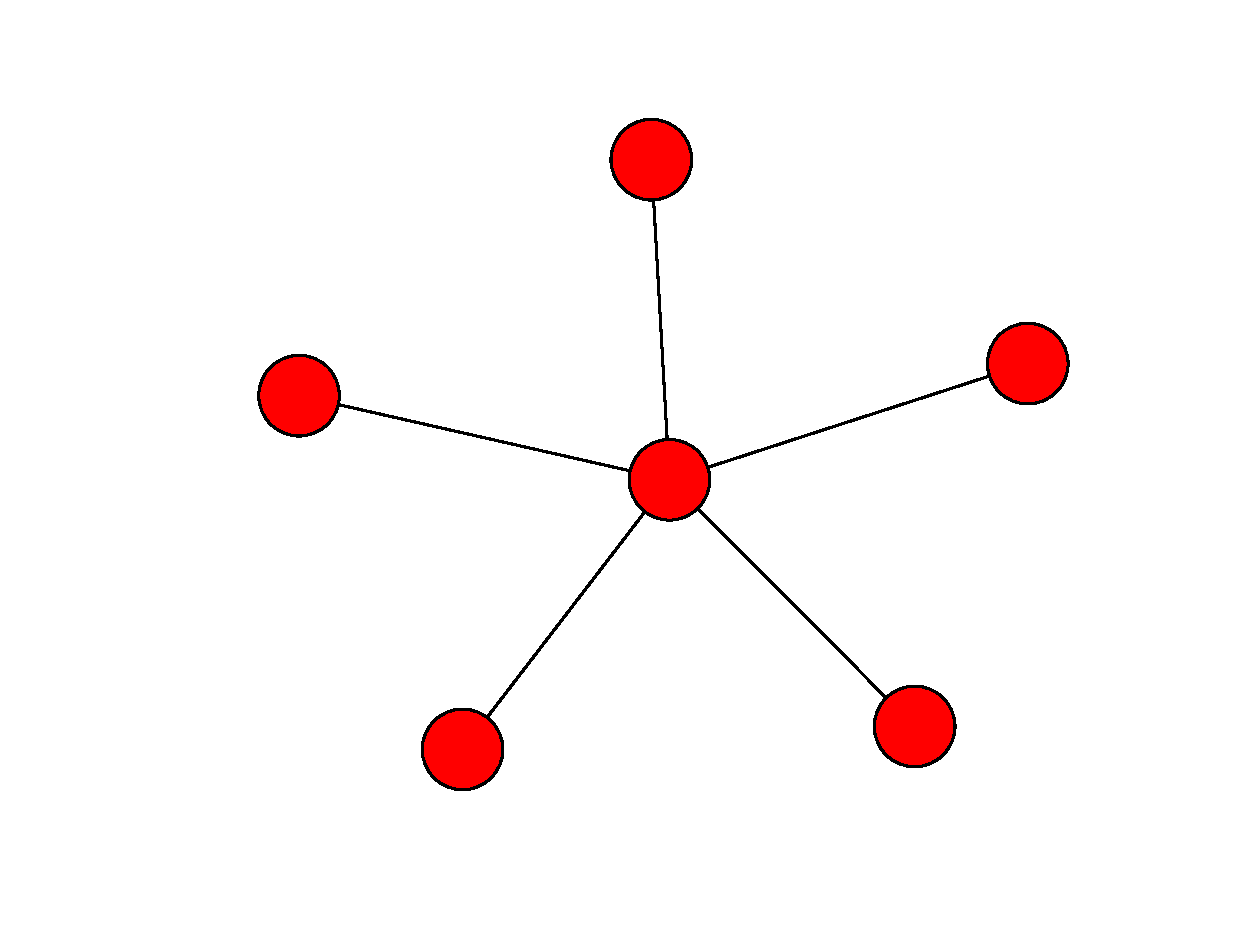
\includegraphics[scale=0.1]{img/star}
\end{center}

\begin{center}
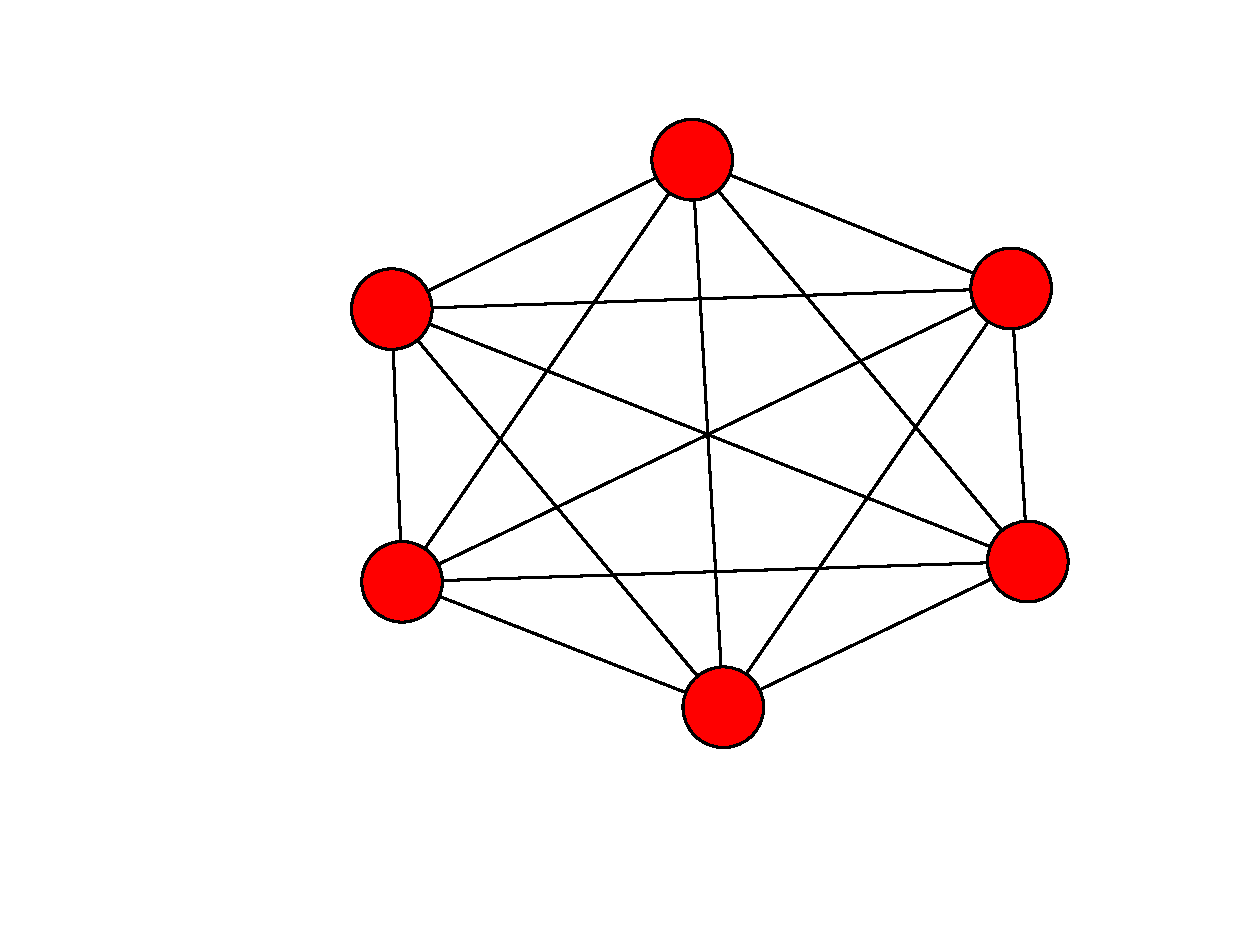
\includegraphics[scale=0.1]{img/complete}
\end{center}
\end{column}

\begin{column}{0.3\textwidth}
\textbf{Overlap} a cohesion measure should allow some actors to be part of more than one cohesive subgroup.

\begin{center}
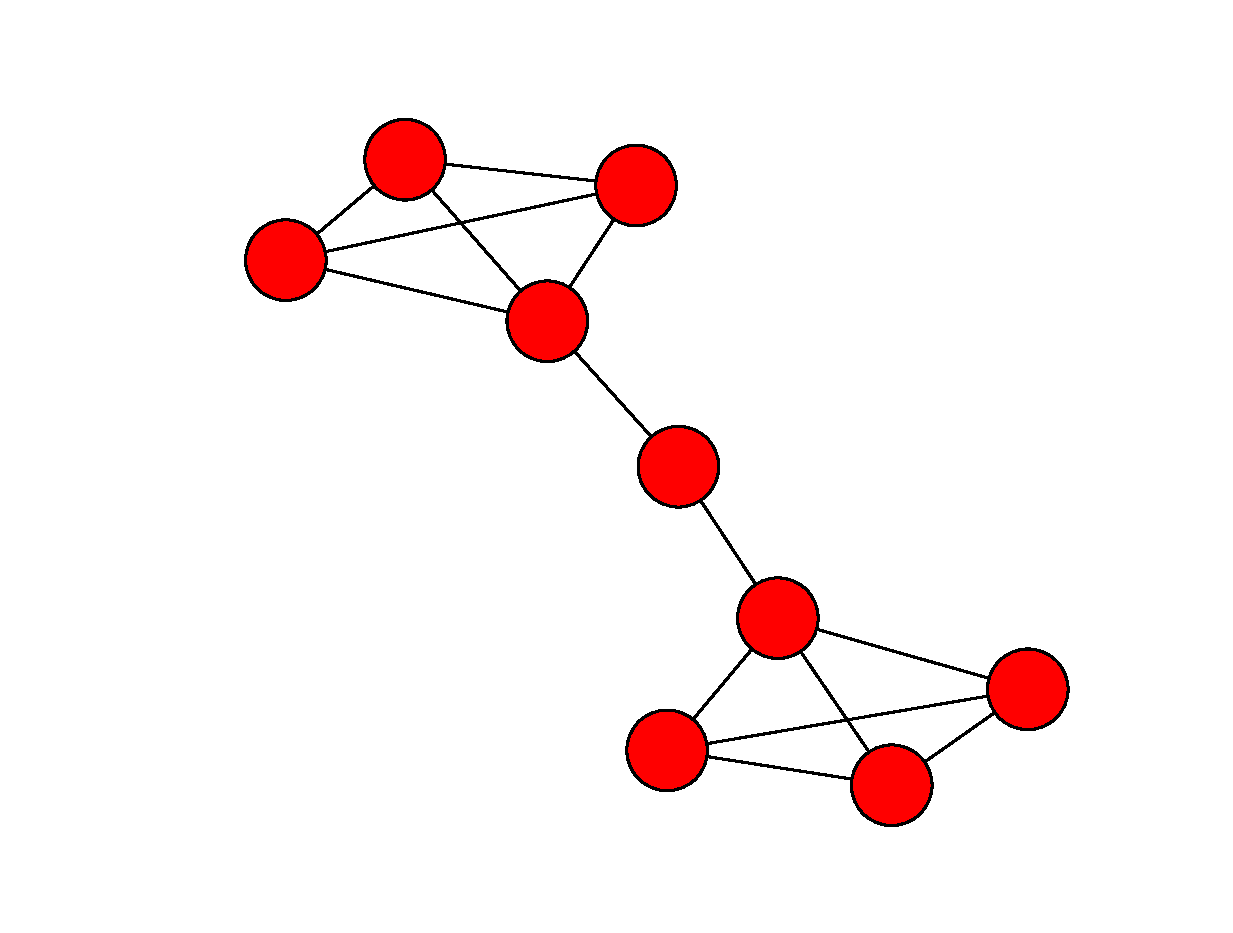
\includegraphics[scale=0.1]{img/hole}
\end{center}

\begin{center}
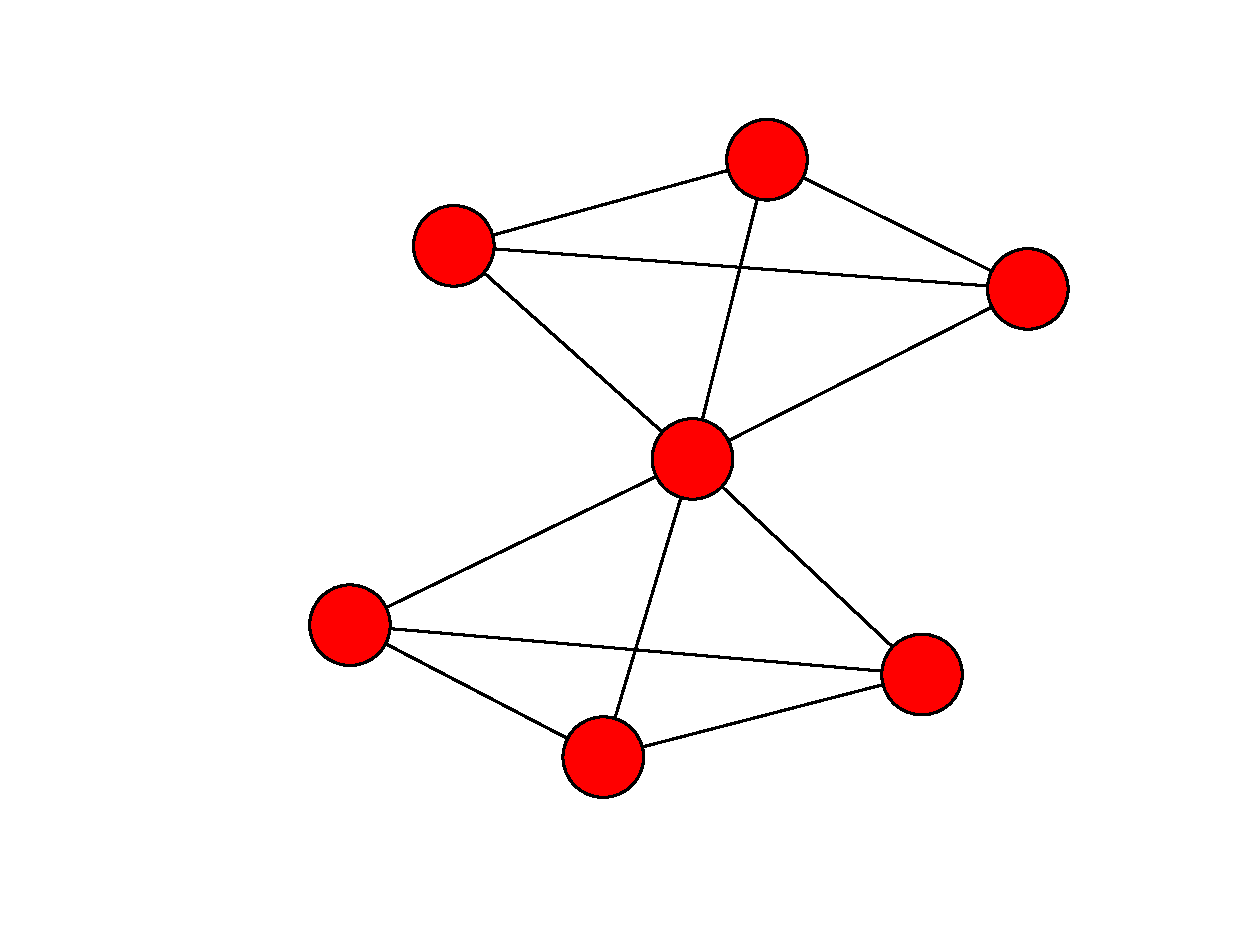
\includegraphics[scale=0.1]{img/fold}
\end{center}
\end{column}

\begin{column}{0.4\textwidth}
\textbf{Hierarchical} highly cohesive subgroups are nested inside less cohesive ones.

\begin{center}
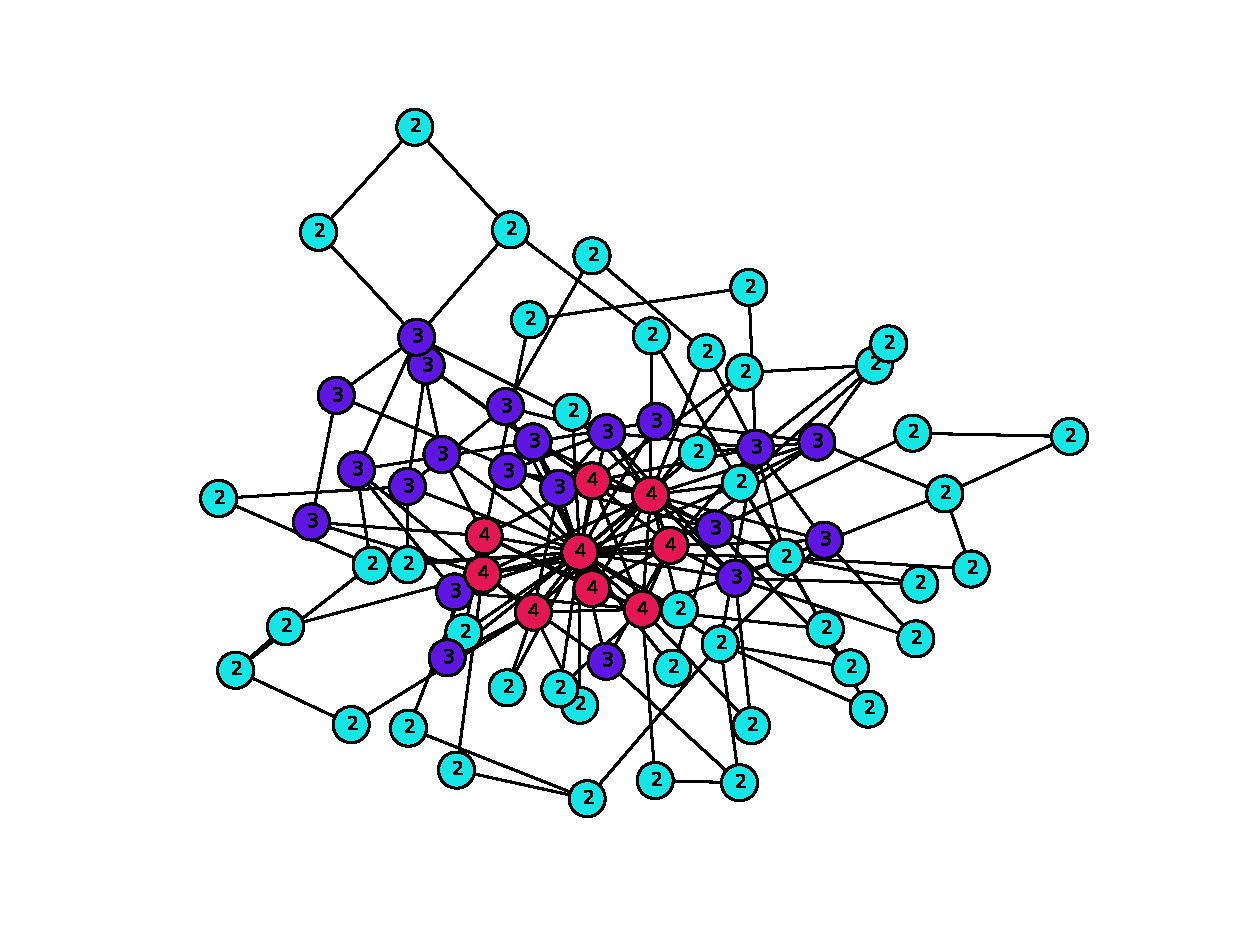
\includegraphics[scale=0.25]{img/knum_colors}
\end{center}
\end{column}

\end{columns}

\end{frame}

\subsection{Structural cohesion model}

\begin{frame}
\frametitle{The structural cohesion model}

The structural cohesion model \citep{white:2001,moody:2003} is based on two mathematically equivalent definitions of cohesion.

\begin{block}{Precise definition of group cohesion based on \textbf{node connectivity}}

\begin{itemize}

\item a group's structural cohesion is equal to the minimum number of actors who, if removed from the group, would disconnect the group.

\item a group's structural cohesion is equal to the minimum number of node independent paths linking each pair of actors in the group.

\end{itemize}
\end{block}

This equivalence relation has a deep sociological meaning because it allows to define structural cohesion in terms of:

\begin{itemize}

\item the difficulty to pull a group apart by removing actors.

\item multiple relations between actors that keep a group together.

\end{itemize}
\end{frame}

\begin{frame}
\frametitle{Measures of structural cohesion}

\begin{block}{Node connectivity $\kappa(G)$}
\begin{description}
\item[Local] given two nodes $u$ and $v$, $\kappa_{G}(u,v)$ is the minimum number of nodes that must be removed to destroy all paths that join $u$ and $v$.

\item[Global] the minimum number of nodes that must be removed in order to disconnect a graph $G$.

\begin{equation*}
\kappa = min{\{\kappa_{G}(u,v):u,v \in V(G)\}}
\end{equation*}

\end{description}

\end{block}

\begin{block}{Average node connectivity $\bar{\kappa}(G)$}
the sum of local node connectivity between all pairs of different nodes of $G$ divided by the number of distinct pairs of nodes. \citep*{beineke:2002}.

\begin{equation*}
\bar{\kappa}(G) = \frac{\sum_{u,v} \kappa_{G}(u,v)}{{n \choose 2}}
\end{equation*}
\end{block}

\begin{block}{$k$-components}
A $k$-component is a maximal subgraph that has, at least, node connectivity $k$: we need to remove at least $k$ nodes to break it into more components. 
\end{block}

\begin{center}
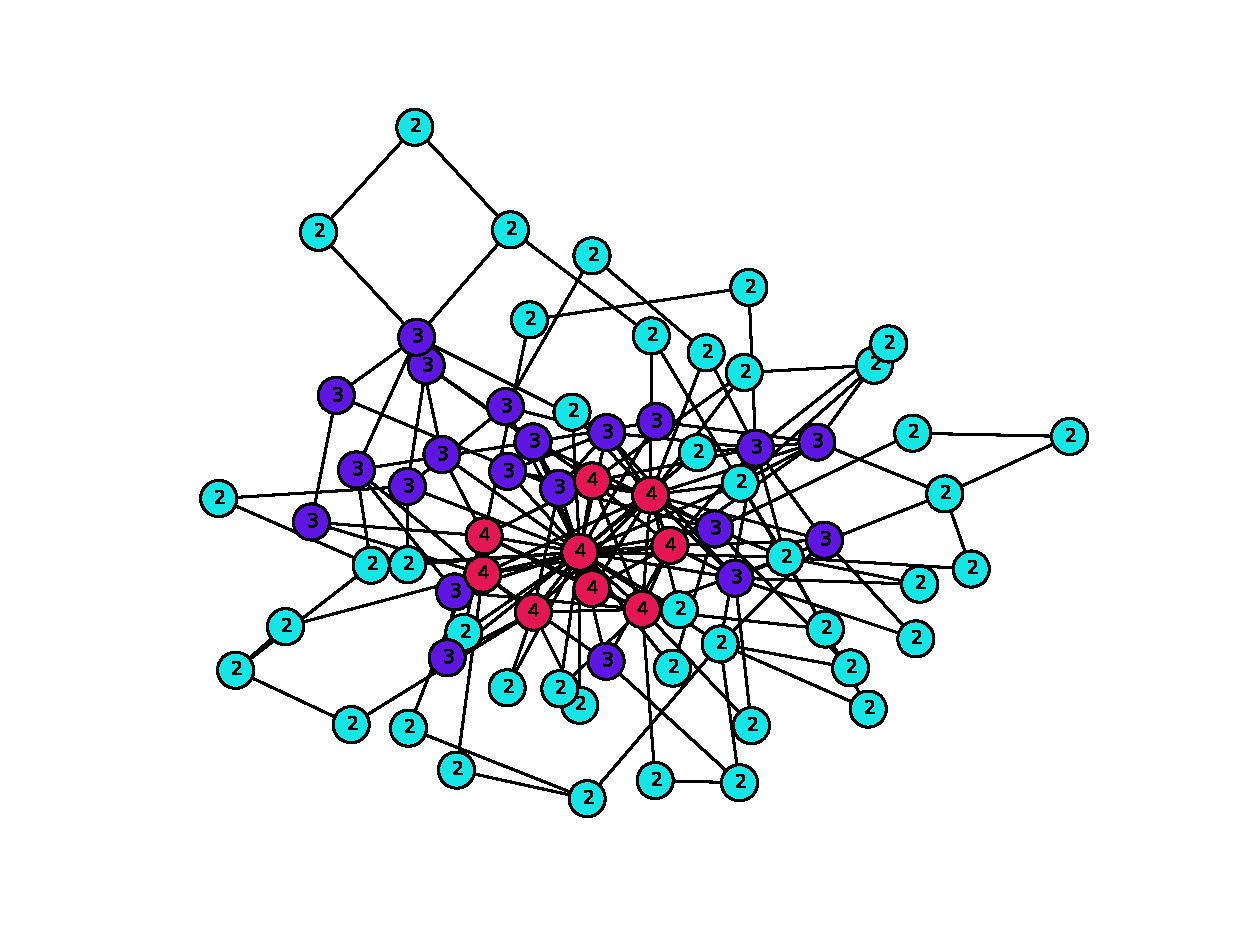
\includegraphics[scale=0.25]{img/knum_colors}
\end{center}

\end{frame}

\begin{frame}
\frametitle{Structural cohesion in empirical analysis}

Structural cohesion is a powerful and robust explanatory factor for a wide variety of interesting empirical social phenomena: 

\begin{itemize}

\item likelihood of building alliances and partnerships among biotech firms \citep{powell:2005}

\item school attachment and academic performance of young people and the tendency of firms to enroll in similar political activity behaviors \citep{moody:2003}

\item emerging trust relations among neighborhood residents and the hiring relations among top level US graduate programs \citep{grannis:2009}

\end{itemize}

\begin{block}{Some problems with the structural cohesion model}

Despite all its merits, the structural cohesion model has not been widely applied to empirical analysis because:

\begin{itemize}

\item it is not practical to compute it for networks with more than a few hundreds nodes and edges due to its computational complexity.

\item it is not implemented in most popular network analysis software packages.

\end{itemize}
\end{block}
\end{frame}

\subsection{Algorithms and Heuristics}

\subsubsection{Exact algorithm for structural cohesion}

\begin{frame}[fragile]
\frametitle{Exact Algorithm}

\citet[appendix A]{moody:2003} provide an algorithm for identifying $k$-components in a network, which is based on the \citet{kanevsky:1993} algorithm for finding all minimum-size node cut-sets of a graph.

\begin{enumerate}

\item Identify the node connectivity, $k$, of the input graph.

\item Identify all $k$-cutsets at the current level of connectivity.

\item Generate new graph components based on the removal of these cutsets.

\item If the graph is neither complete nor trivial, return to 1; otherwise end.

\end{enumerate}


\begin{columns}[c]
\begin{column}{0.4\textwidth}
\begin{scriptsize}
\begin{lstlisting}
import networkx as nx
from networkx import convert_node_labels_to_integers as cnlti

G = cnlti(nx.grid_2d_graph(5,5))
list(nx.all_node_cuts(G))
[{1, 9}, {22, 23}, {17, 18}, {3, 14}]
# To compute k-components
kcomponents = nx.k_components(G)
\end{lstlisting}
\end{scriptsize}

\end{column}

\begin{column}{0.6\textwidth}
\begin{center}
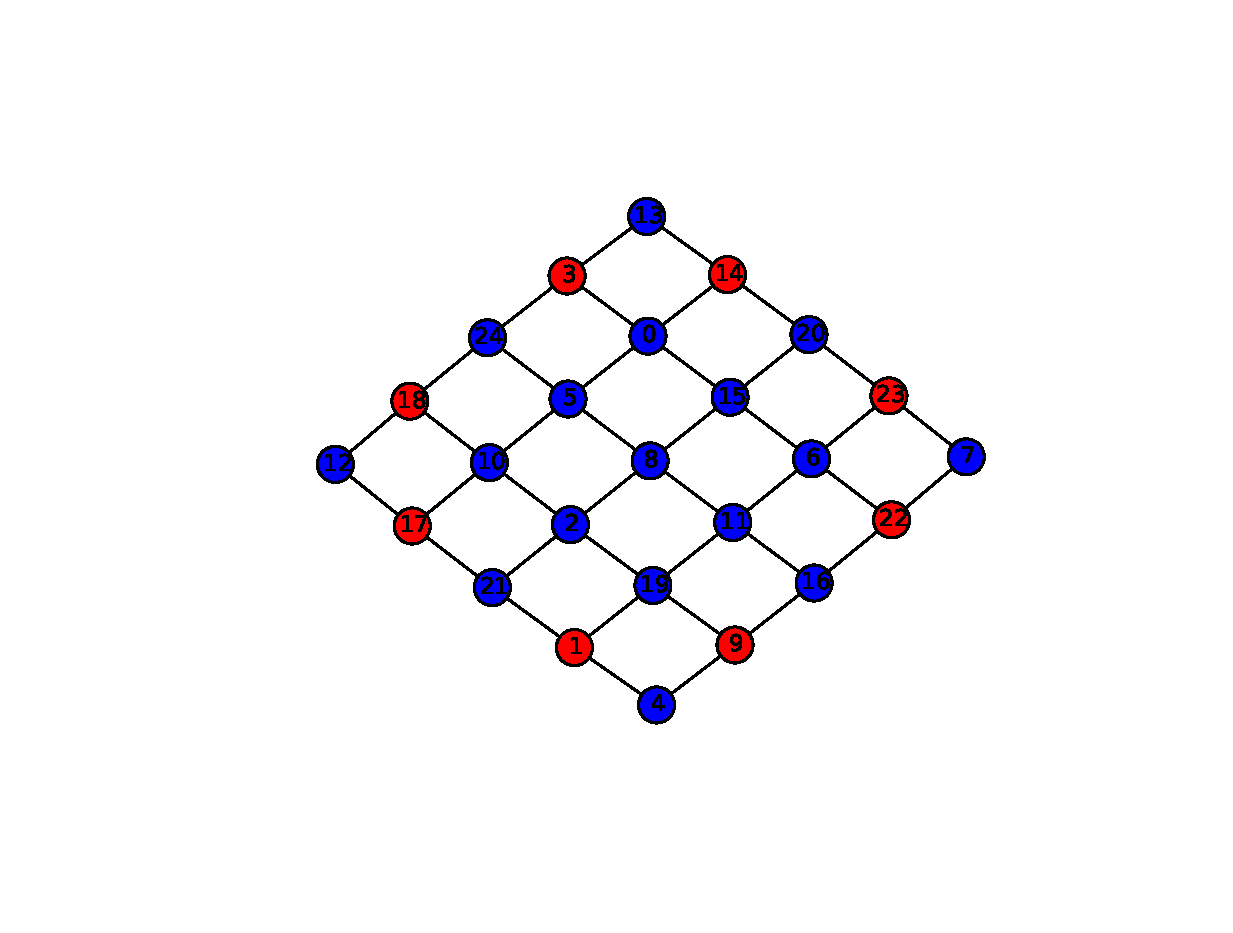
\includegraphics[scale=0.45]{img/grid}
\end{center}

\end{column}
\end{columns}

\end{frame}

\subsubsection{Heuristics for computing structural cohesion}

\begin{frame}[fragile]
\frametitle{Heuristics}

The heuristics we developed are based on:

\begin{block}{Approximation to local node connectivity}
\citet{white:2001b} fast approximation algorithm for finding good lower bounds of the number of node independent paths between two nodes.

\begin{columns}[c]
\begin{column}{0.1\textwidth}

\end{column}

\begin{column}{0.8\textwidth}
\begin{scriptsize}
\begin{lstlisting}
import networkx as nx
from networkx.algorithms import approximation as apxa
# Exact computation of node connectivity
exact = nx.node_connectivity(G)
# Lower bound approximation
aprox = apxa.node_connectivity(G)
\end{lstlisting}
\end{scriptsize}
\end{column}

\begin{column}{0.1\textwidth}

\end{column}
\end{columns}
\end{block}

\begin{block}{Whitney's theorem}
inclusion relation among node connectivity $\kappa(G)$, edge connectivity $\lambda(G)$ and minimum degree $\delta(G)$ for any graph $G$:

\begin{equation*}
\kappa(G) \le \lambda(G) \le \delta(G)
\end{equation*}

``$k$-cores can be regarded as seedbeds, within which we can expect highly cohesive subsets to be found'' \citet[281]{seidman:1983}
\end{block}
\end{frame}

\begin{frame}
\frametitle{Heuristics}

\begin{block}{Main logic of the heuristics}

\begin{enumerate}

\item repeatedly applying fast algorithms for $k$-cores \citep{batagelj:2011} and biconnected components \citep{tarjan:1972} in order to narrow down the number of pairs of different nodes over which we have to compute their local node connectivity.

\item Build an auxiliary graph $H$ in which two nodes are linked if they have at least $k$ node independent paths connecting them.

\item Complete subgraphs in $H$ have a one to one correspondence with subgraphs of $G$ in which each node is connected to every other node in the subgraph for at least $k$ node independent paths. That is, $k$-components.

\end{enumerate}
\end{block}

\begin{block}{Trade Accuracy for Speed}
\begin{tiny}
\begin{tabular}{|c|c|c|c|c|c|c|c|c|}
\hline
&\multicolumn{4}{|c|}{Bipartite}&\multicolumn{4}{|c|}{Unipartite}\\
Network&\# nodes&\# edges&Av. degree&Time(s)&\# nodes&\# edges&Av. degree&Time(s)\\
\hline
Debian Lenny&13,121&20,220&3.08&1,105.2&1,383&5,216&7.54&204.7\\
High Energy (theory)&26,590&37,566&2.81&3,105.7&9,767&19,331&3.97&7,136.0\\
Nuclear Theory&10,371&15,969&3.08&1,205.2&4,827&14,488&6.00&3,934.1\\
\hline
\end{tabular}
\end{tiny}
\end{block}

\end{frame}



\section{The Network Structure of Collaborative Communities}

\begin{frame}
\frametitle{Collaborative Communities}
A new form of community, qualitatively different from the traditional \emph{Gemeinschaft} and the modern \emph{Gesellschaft} \citep{tonnies:1974}. 

\begin{block}{Collaborative Communities \citep{adler:2006}}
Novel organizational form ---both inside and outside large capitalist corporations--- strongly grounded on large scale cooperation which defy the traditional dichotomy between \textbf{hierarchy} and \textbf{market} as coordinating mechanisms.

\begin{itemize}
\item Generalized trust based on other's contributions towards a shared end.
\item Conscious cooperation and high individual interdependence.
\item Shared values and value-rational basis for legitimate authority. 
\end{itemize}
\end{block}

So far scarce attention is given to the structural features of collaborative communities.

\begin{description}
\item[Question] explore the network structure that lead to their emergence and effectiveness in the production and diffusion of knowledge.

\item[Contribution] I suggest that a unique network structure undergirds collaborative communities and build a model to understand its key mechanisms: the \textbf{cohesive small world} model.
\end{description}

\end{frame}


\begin{frame}
\frametitle{knowledge-based production processes}
Collaborative Communities are especially well suited to deal with the challenges of knowledge-based production processes because, hierarchy and market have proved ineffective, at best, at managing knowledge.  

\begin{columns}[c]

\begin{column}{0.5\textwidth}
\begin{block}{Hierarchy as a coordinating mechanism}
\begin{itemize}
\item Knowledge is treated as a scare resource.
\item Centralized at the higher levels where key decisions are taken.
\item Rigidity prevents flexibility to deal with unanticipated problems.
\item Difficulty to foster innovation and generation of new knowledge.
\end{itemize}
\end{block}
\end{column}

\begin{column}{0.5\textwidth}
\begin{block}{Market as coordinating mechanism}
\begin{itemize}
\item Fails to optimize at the same time production and allocation of knowledge.
\item Knowledge is a public good that grow rather than diminish with use.
\item Strong property rights incentive knowledge production, but
\item they block socially optimal allocation (free access).
\end{itemize}
\end{block}
\end{column}

\end{columns}

\begin{block}{Collaborative Communities that excel at knowledge-based production}
\begin{itemize}
\item Free and Open Source Communities.
\item Novel forms of professional work organization \citep*{adler:2008}.
\item Knowledge-intensive production processes in corporations \citep{adler:2006}.
\end{itemize}
\end{block}

\end{frame}


\begin{frame}
\frametitle{A network model for Collaborative Communities}

\begin{columns}[c]
\begin{column}{0.5\textwidth}
\begin{block}{The Small World Model}
Networks characterized by a high level of local density of social ties and short average distances among nodes.

\begin{itemize}
\item $L$: average number of intermediaries between any two nodes.
\item $CC$: mean probability that two nodes that are neighbors of the same other node will themselves be neighbors.
\item They foster the flow of information and ideas.

\end{itemize}
\end{block}
\end{column}

\begin{column}{0.5\textwidth}
\begin{block}{The Structural Cohesion Model}
Networks characterized by the presence of increasingly cohesive groups nested inside each other. 
\begin{itemize}
\item Cohesion definition based on the graph-theoretic property of connectivity.
\item $k$-components as the key subgroups of the network.
\item They foster the development of trust and social cohesion.
\end{itemize}
\end{block}
\end{column}

\end{columns}

These two models are not mutually exclusive. The networks that fit in the intersection of both models exhibit consistent structural patterns.

\begin{block}{Cohesive Small World Model}
Network (structural) model for Collaborative Communities that help explain how trust, value congruence, and large scale cooperation are enabled and fostered.

\begin{itemize}
\item Local clusters connected by short paths.
\item Increasingly cohesive groups nested inside each other.
\end{itemize}
\end{block}

These patterns provide the structural scaffolding for collaborative communities.

\note{On the one hand, the generation of trust and congruent values among heterogeneous individuals are fostered by structurally cohesive groups in the connectivity hierarchy of cooperation networks because individuals embedded in these structures are able to compare independent perspectives on each other through a variety of relations that flow through distinct sets of intermediaries, which provides multiple independent sources of information about each other. Thus, the perception of an individual embedded in such structures of the other members of the group to whom she is not directly linked is filtered by the perception of a variety of others whom she trusts because is directly linked to them. This mediated perception of the group generates trust at a global scale. On the other hand, the existence of dense local clusters connected between them by relative short paths allows successful cooperation among heterogeneous individuals with common interests and, at the same time, fosters the flow of information between these clusters preventing the local clusters to be trapped in echo chambers of like minded collaborators.}

\end{frame}

\subsection{Cohesive Small Worlds}

\begin{frame}
\frametitle{Cohesive Small World}

\begin{columns}[c]
\begin{column}{0.33\textwidth}
\begin{center}
\textbf{Pure Structural Cohesion}
\end{center}
\begin{itemize}
\item Robust to node removal
\item Not necessary short average distance
\item Not necessary local clustering 
\end{itemize}
\includegraphics[scale=0.2]{../../figures/model_structural_cohesion_25}
\end{column}

\begin{column}{0.33\textwidth}
\begin{center}
\textbf{Cohesive Small World}
\end{center}
\begin{itemize}
\item Intersection of the two models
\item Short average distance
\item High local cluster coefficient
\item Robust to node removal
\end{itemize}
\includegraphics[scale=0.2]{../../figures/model_cohesive_small_world_25}
\end{column}

\begin{column}{0.33\textwidth}
\begin{center}
\textbf{Pure Small World}
\end{center}
\begin{itemize}
\item Short average distance
\item High local cluster coefficient
\item Not necessary robust to node removal
\end{itemize}
\includegraphics[scale=0.2]{../../figures/model_small_world_25}
\end{column}
\end{columns}

\end{frame}


\section{Empirical analysis: FOSS projects}

\subsection{Debian and Python}

\begin{frame}
\frametitle{Free and Open Source Projects: Debian and Python}

Free Software, broadly defined, is computer software that allows users to run, copy, distribute, study, change and improve it.

\begin{columns}[c]
\begin{column}{0.5\textwidth}
\begin{block}{The Debian Project: 1999-2012}
\begin{itemize}
\item A free Operating System
\item 392 developers in 1999, 1435 in 2012 
\item 2876 programs in 1999, 10469 in 2012
\item Widely used in servers (google), desktops (Ubuntu) and embedded devices (raspberry pi)
\end{itemize}
\end{block}
\end{column}

\begin{column}{0.5\textwidth}
\begin{block}{The Python project: 1999-2014}
\begin{itemize}
\item A free Programming Language
\item 9 developers in 1999, 62 in 2014
\item 1137 files in 1999, 2134 in 2014 
\item Widely used in web development (reddit, youtube) and scientific computing
\end{itemize}
\end{block}
\end{column}
\end{columns}

\begin{block}{}
\begin{itemize}
\item 
\item 
\item 
\end{itemize}
\end{block}

\end{frame}

\subsection{Cooperation Networks and Null Models}

\begin{frame}
\frametitle{Cooperation Networks and Null Models}

My modeling strategy to capture the patterns of relations among developers in these two projects is to focus on the actual contributions of each developer to the project. 

\begin{block}{Building Cooperation Networks}
\begin{itemize}
\item Focus on the patterns of relations among developers in the productive process.
\item Cooperation networks are bipartite or two mode; node sets are developers and programs/files and edges only link nodes from opposite sets.
\item A developer is linked to the package (in Debian) or source code file (in Python) that she works on.
\item We have complete electronic records of all package uplads to Debain and all sorce code file edits in Python.
\end{itemize}
\end{block}

\begin{block}{Building Suitable Null models}
\begin{itemize}
\item We need to compare the statistical measures obtained from the actual networks with a suitable null model in order to assert that what we observe is not the result of pure chance.
\end{itemize}
\begin{description}
\item [Configuration Model] assigns at random developers to packages, or developers to source code files, maintaining the concrete skewed distribution of packages by developer and files by developer observed in the actual networks. That is, the degree distribution.
\end{description}
\end{block}

\end{frame}

\subsection{Small World Analysis}

\begin{frame}
\frametitle{Small World Analysis}

A network fits the small world model if it is more locally clustered ($CC$) than its random network counterpart but has approximately the same average distance ($L$) between nodes. 

\begin{align}
Q = \frac{CC_{ratio}}{L_{ratio}} \nonumber & \hspace{0.5cm} \textit{Where:} & 
CC_{ratio}& = \frac{CC_{actual}}{CC_{random}} \nonumber &
L_{ratio}& = \frac{L_{actual}}{L_{random}} \nonumber \\
\end{align}

If the Small World Index ($Q$) is greater than 1, then the network fits the model. 

\begin{columns}[c]
\begin{column}{0.5\textwidth}
\begin{block}{The Debian Project: 1999-2012}
\begin{itemize}
\item $CC_{actual} \gg CC_{random}$ for all years.
\item $L_{actual} > L_{random}$ for all years.
\item $Q \gg 1$ for all years (21.4 in 2011 to 97 in year 2000).
\end{itemize}
\end{block}
\end{column}

\begin{column}{0.5\textwidth}
\begin{block}{The Python project: 1999-2014}
\begin{itemize}
\item $CC_{actual} > CC_{random}$ for all years.
\item $L_{actual} \approx L_{random}$ for all years.
\item $Q > 1$ for all years (ranging from 3 in 1999 to 1.3 in 2011).
\end{itemize}
\end{block}
\end{column}
\end{columns}

\vspace{0.3cm}

The low value of the Small World Index ($Q$) in the Python project, compared with the values of $Q$ in the Debian project, can be attributed to the lower modularity of Python as a programming language compared with the inherent modularity of the Debian project as an operating system.

\end{frame}


\subsection{Structural Cohesion Analysis}

\begin{frame}
\frametitle{Structural Cohesion Analysis}

Analyze the percentage of nodes in $k$-components in actual networks and in their random counterparts.

For $k \leq 2$ the random null model is the upper bound of component size. Thus a network fits the model if it has more levels ($k$) than its random counterparts and the percentage of nodes for $k \leq 2$ is comparable. 

\begin{columns}[c]
\begin{column}{0.5\textwidth}
\begin{block}{The Debian Project: 1999-2012}
\begin{itemize}
\item For 1-components $|V_{actual}| < |V_{random}|$
\item For 2-components $|V_{actual}| < |V_{random}|$
\item Maximum $k$:\\ $3 \leq max(k_{actual}) \leq 5$ and\\ $2 \leq  max(k_{random}) \leq 3$, but always \\ $max(k_{actual}) > max(k_{random})$. 
\end{itemize}
\end{block}
\end{column}

\begin{column}{0.5\textwidth}
\begin{block}{The Python project: 1999-2014}
\begin{itemize}
\item For 1-components $|V_{actual}| \approx |V_{random}|$
\item For 2-components $|V_{actual}| \approx |V_{random}|$
\item Maximum $k$:\\ $5 \leq max(k_{actual}) \leq 10$ and\\ $3 \leq  max(k_{random}) \leq 7$, but always\\ $max(k_{actual}) > max(k_{random})$. 
\end{itemize}
\end{block}
\end{column}
\end{columns}

\vspace{0.3cm}

The fact that cooperation networks in the Python project are more cohesive than the cooperation networks of the Debian project, can also be attributed in part to the lower modularity of Python as a programming language compared with the inherent modularity of the Debian project as an operating system.

\end{frame}



\begin{frame}
\frametitle{Graphical Representation of the Structural Cohesion Analysis}

\begin{columns}[c]
\begin{column}{0.5\textwidth}
\begin{center}
\textbf{Debian Cooperation Network 2004}
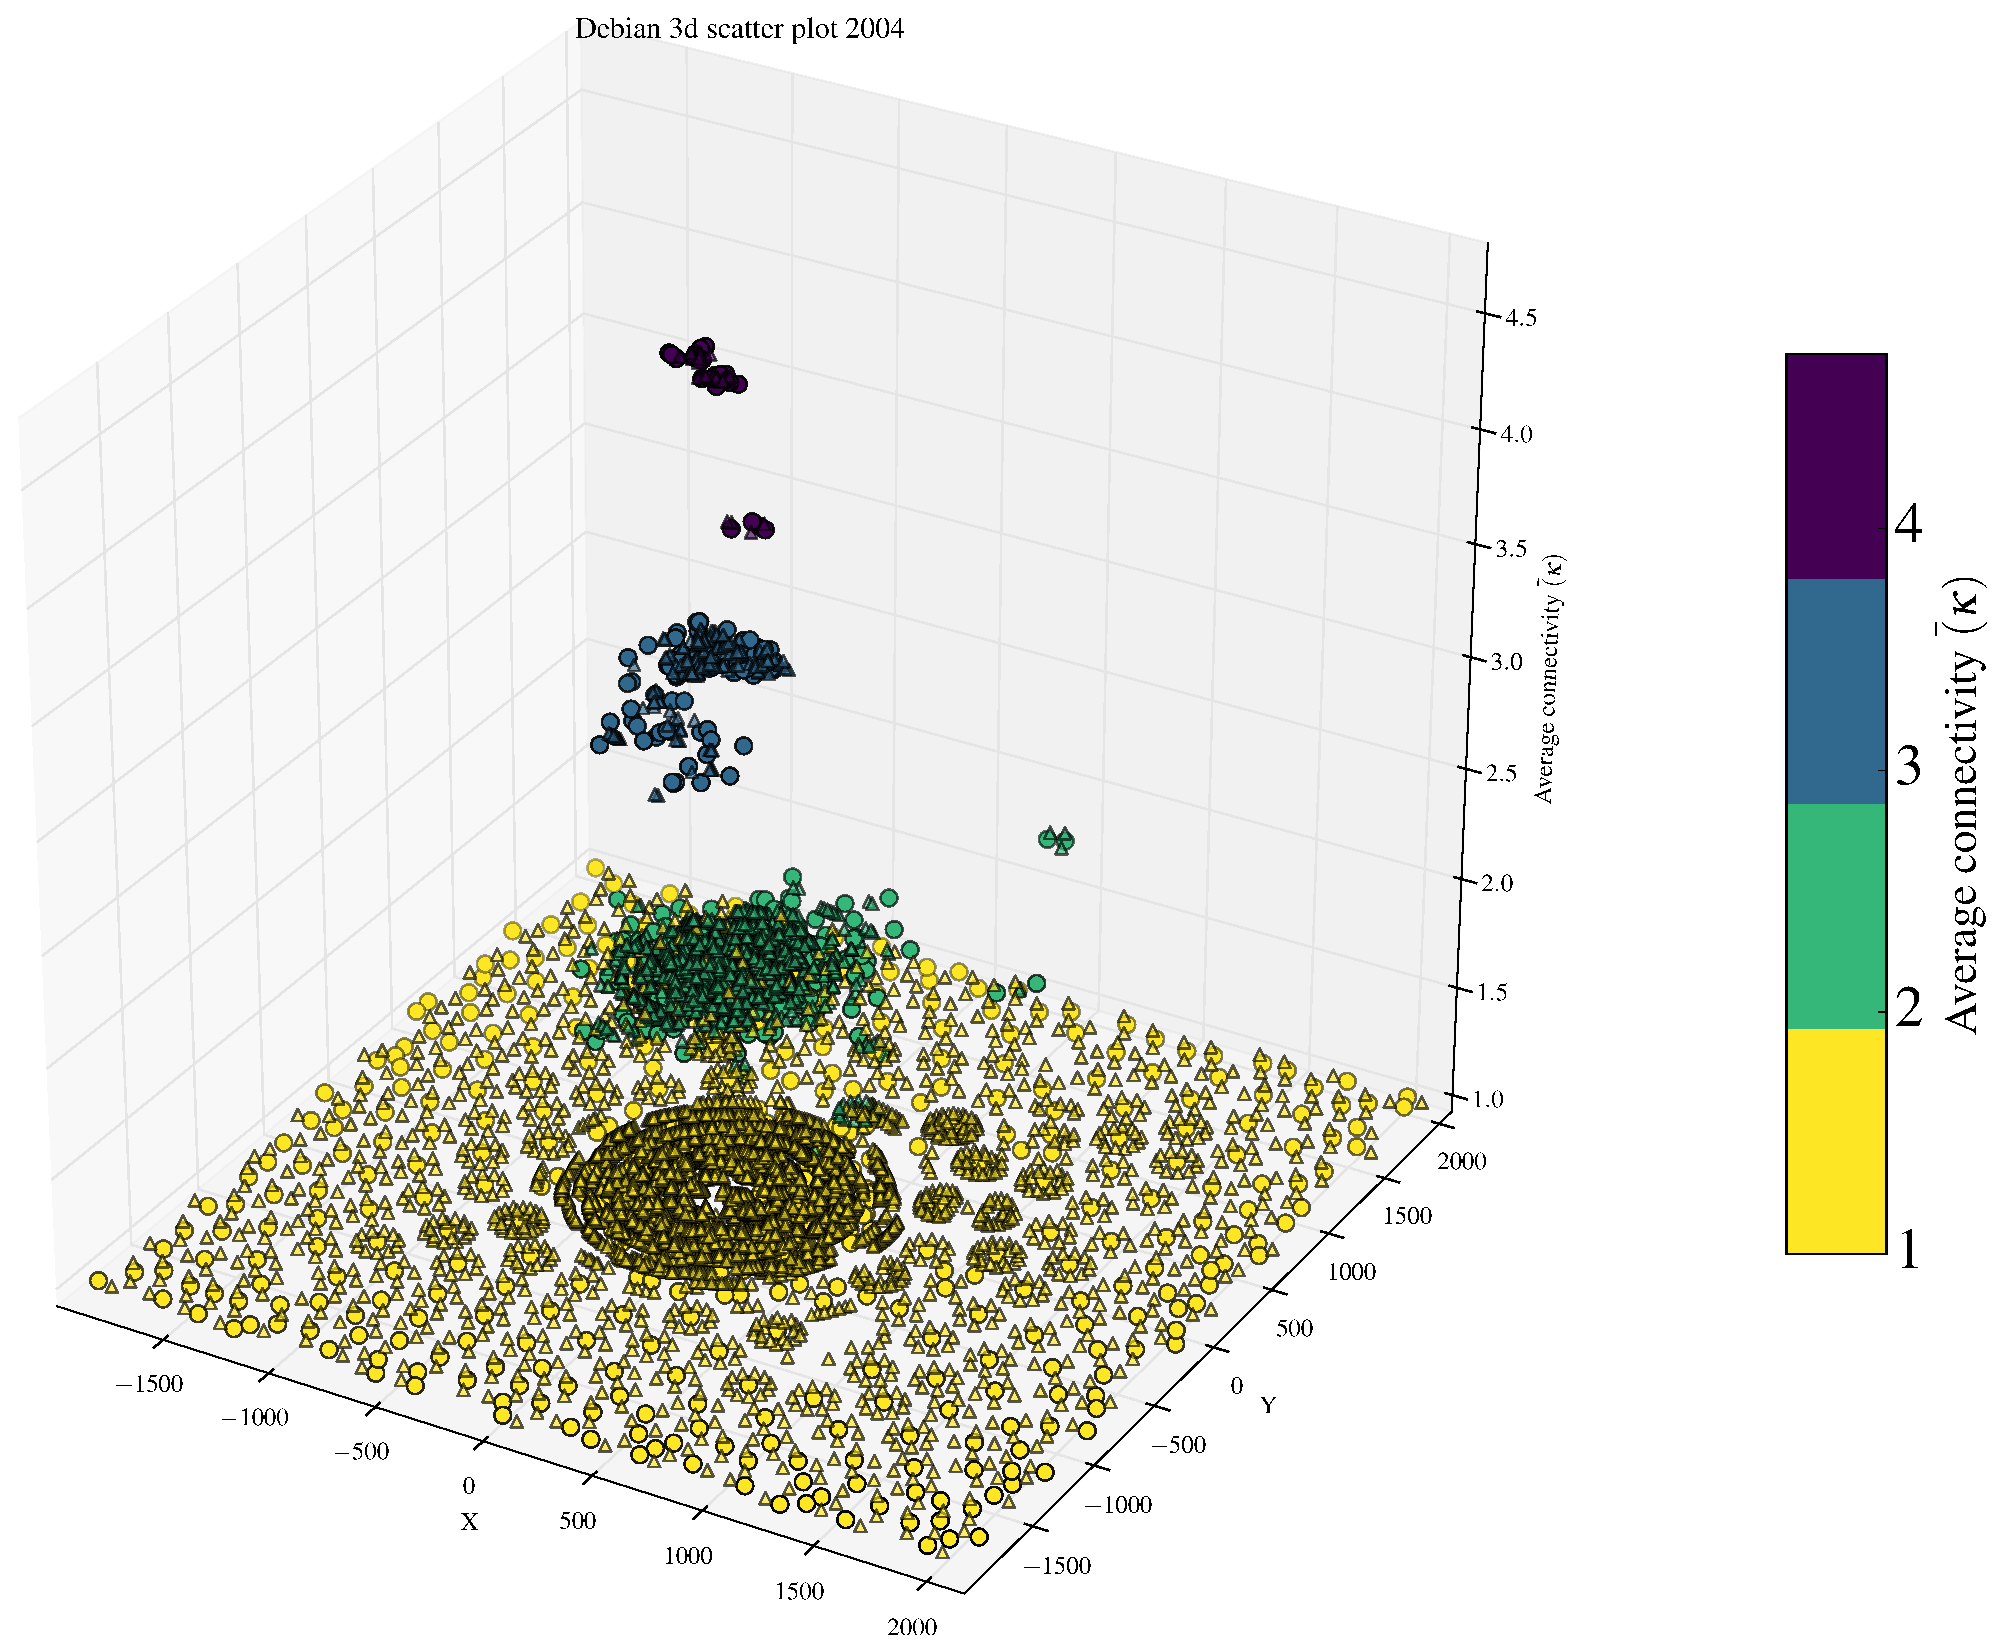
\includegraphics[scale=0.12]{../../figures/3d_scatter_debian_2004}
\newline
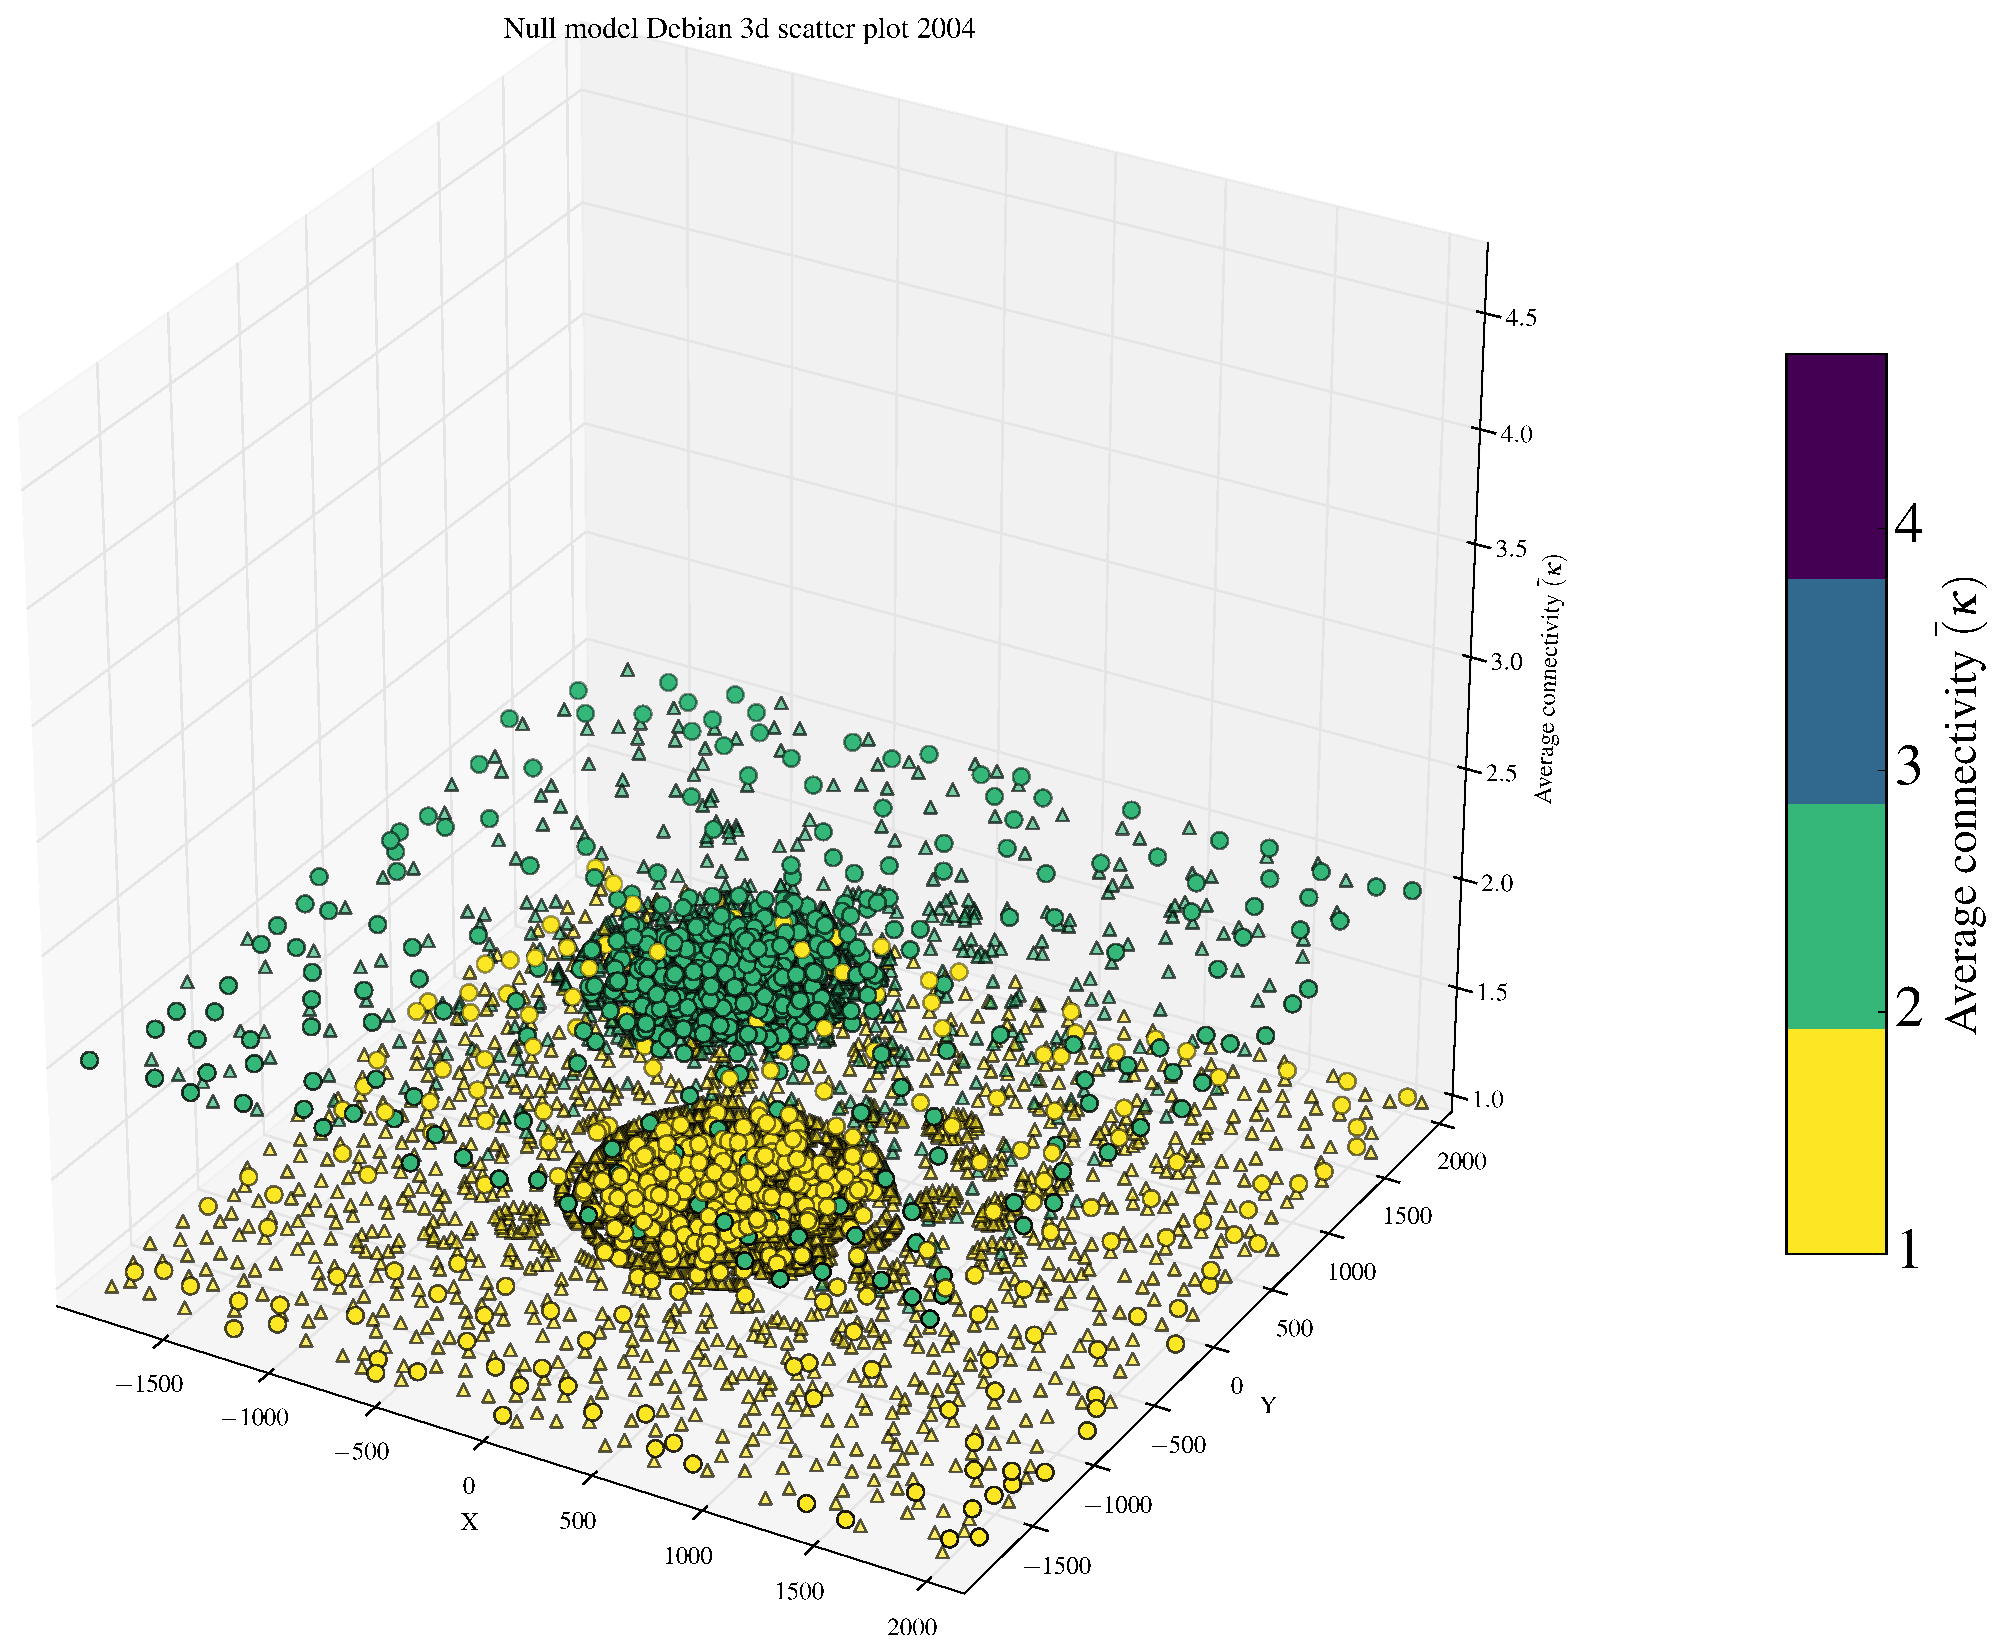
\includegraphics[scale=0.12]{../../figures/3d_scatter_debian_2004_null}
\end{center}
\end{column}

\begin{column}{0.5\textwidth}
\begin{center}
\textbf{Python Cooperation Network 2004}
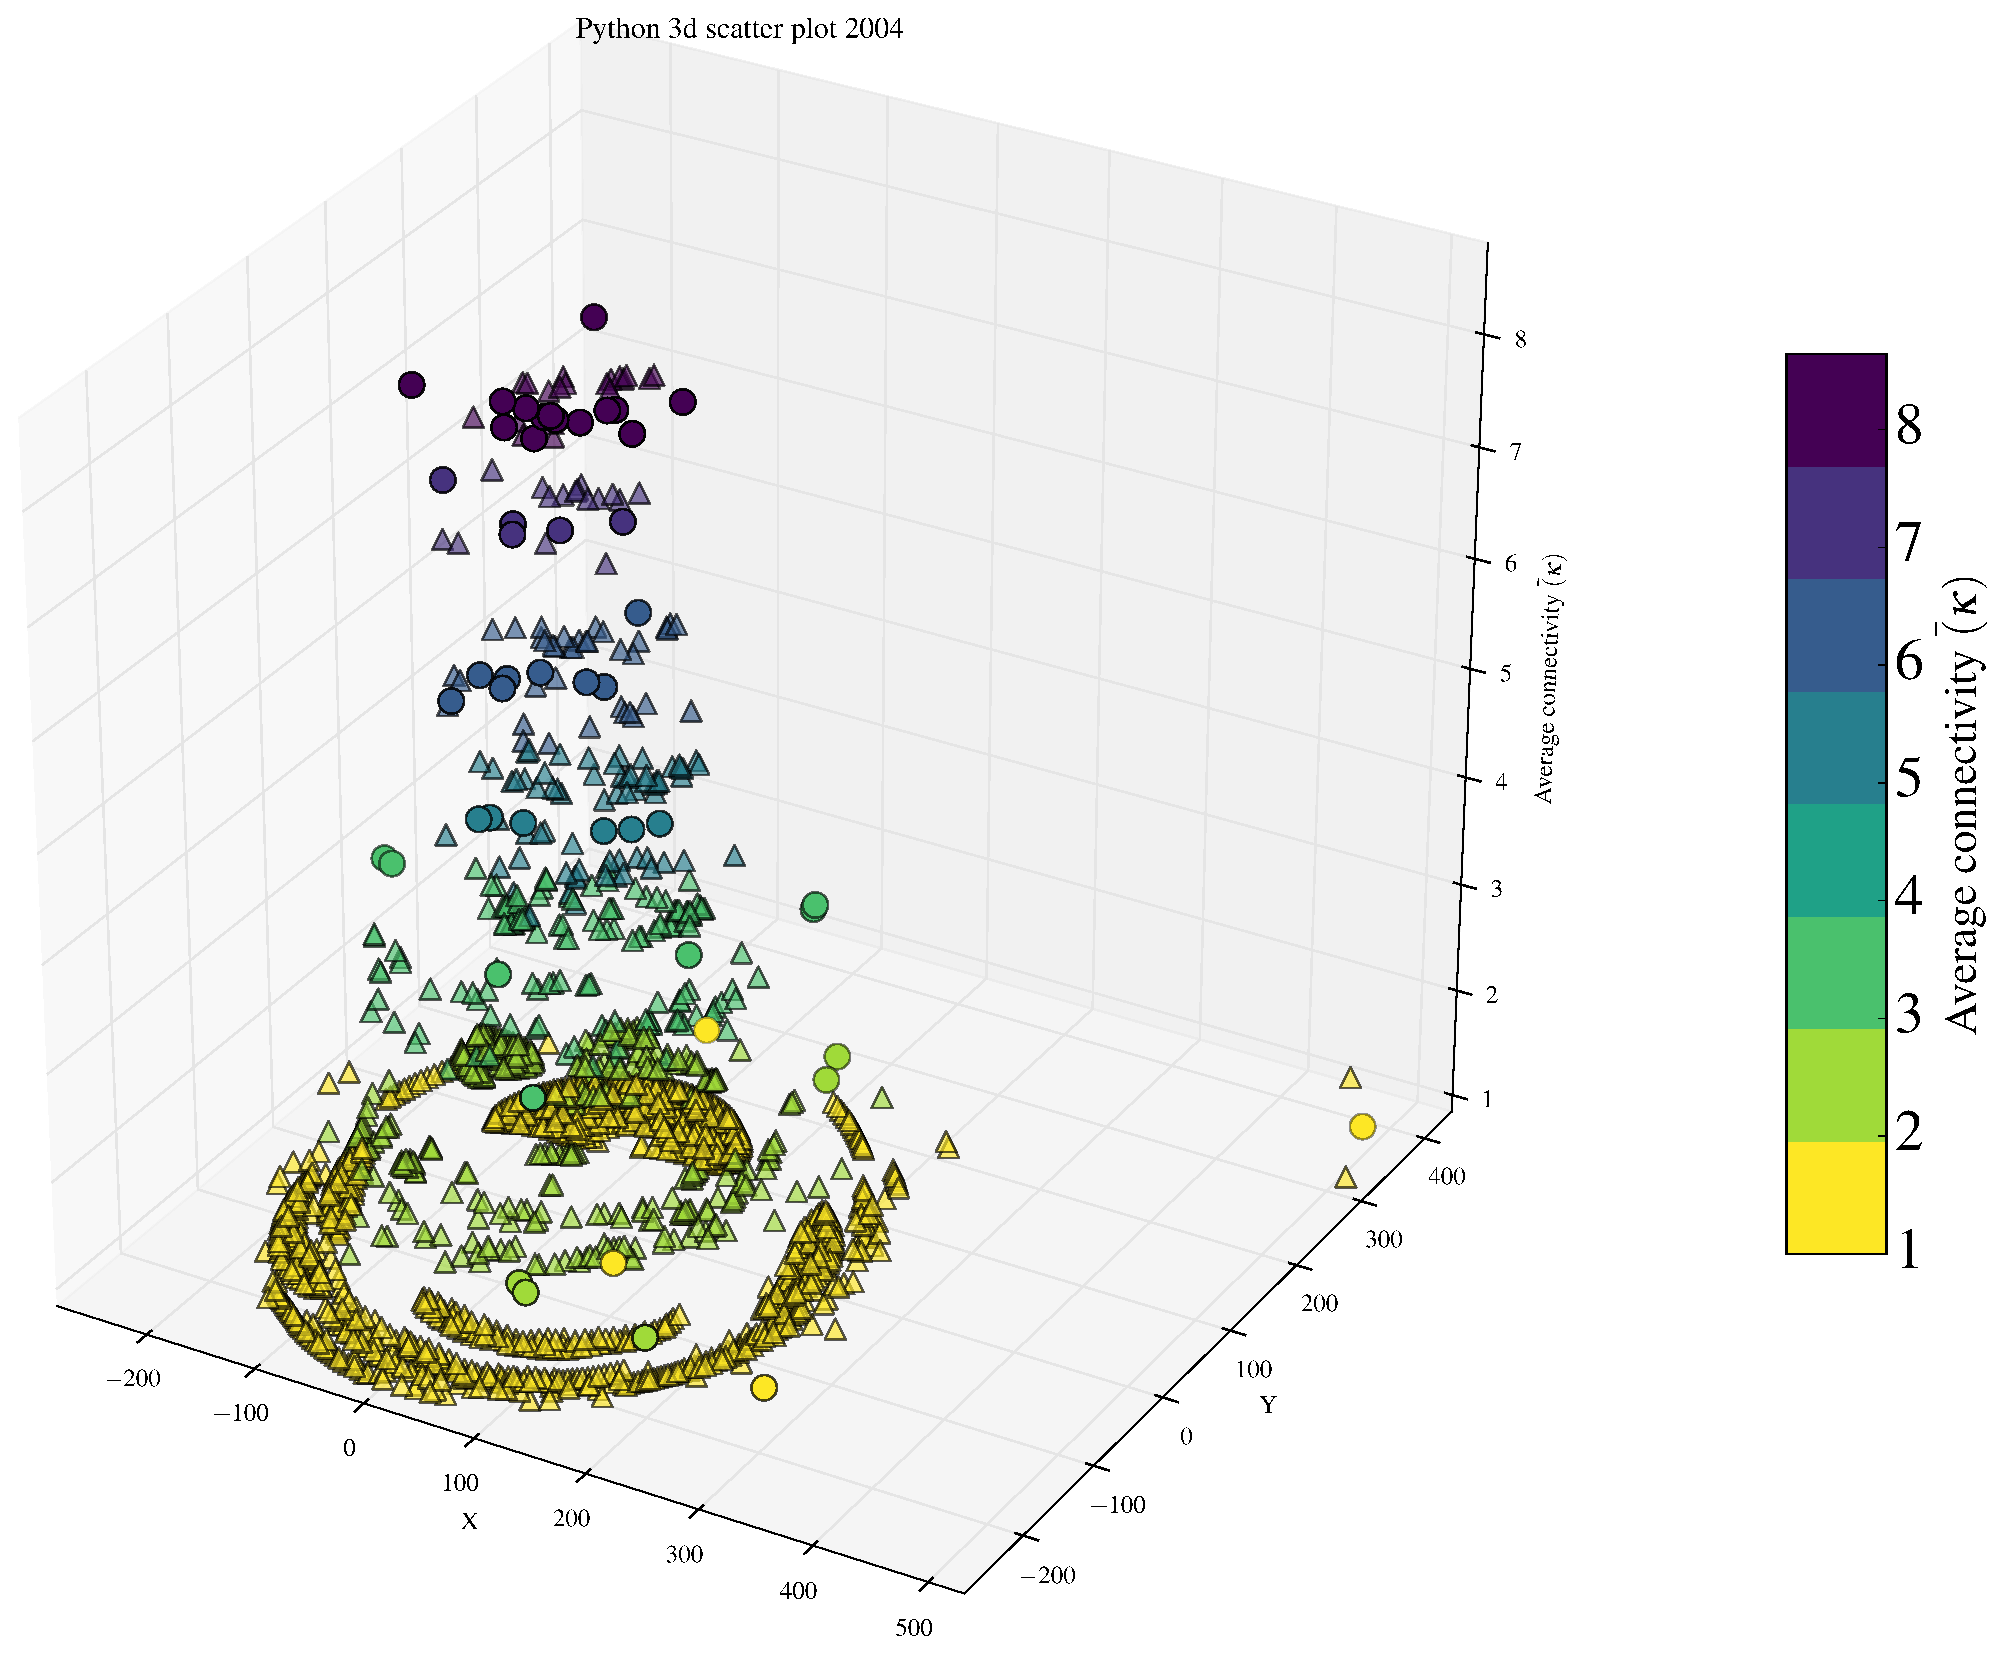
\includegraphics[scale=0.12]{../../figures/3d_scatter_python_2004}
\newline
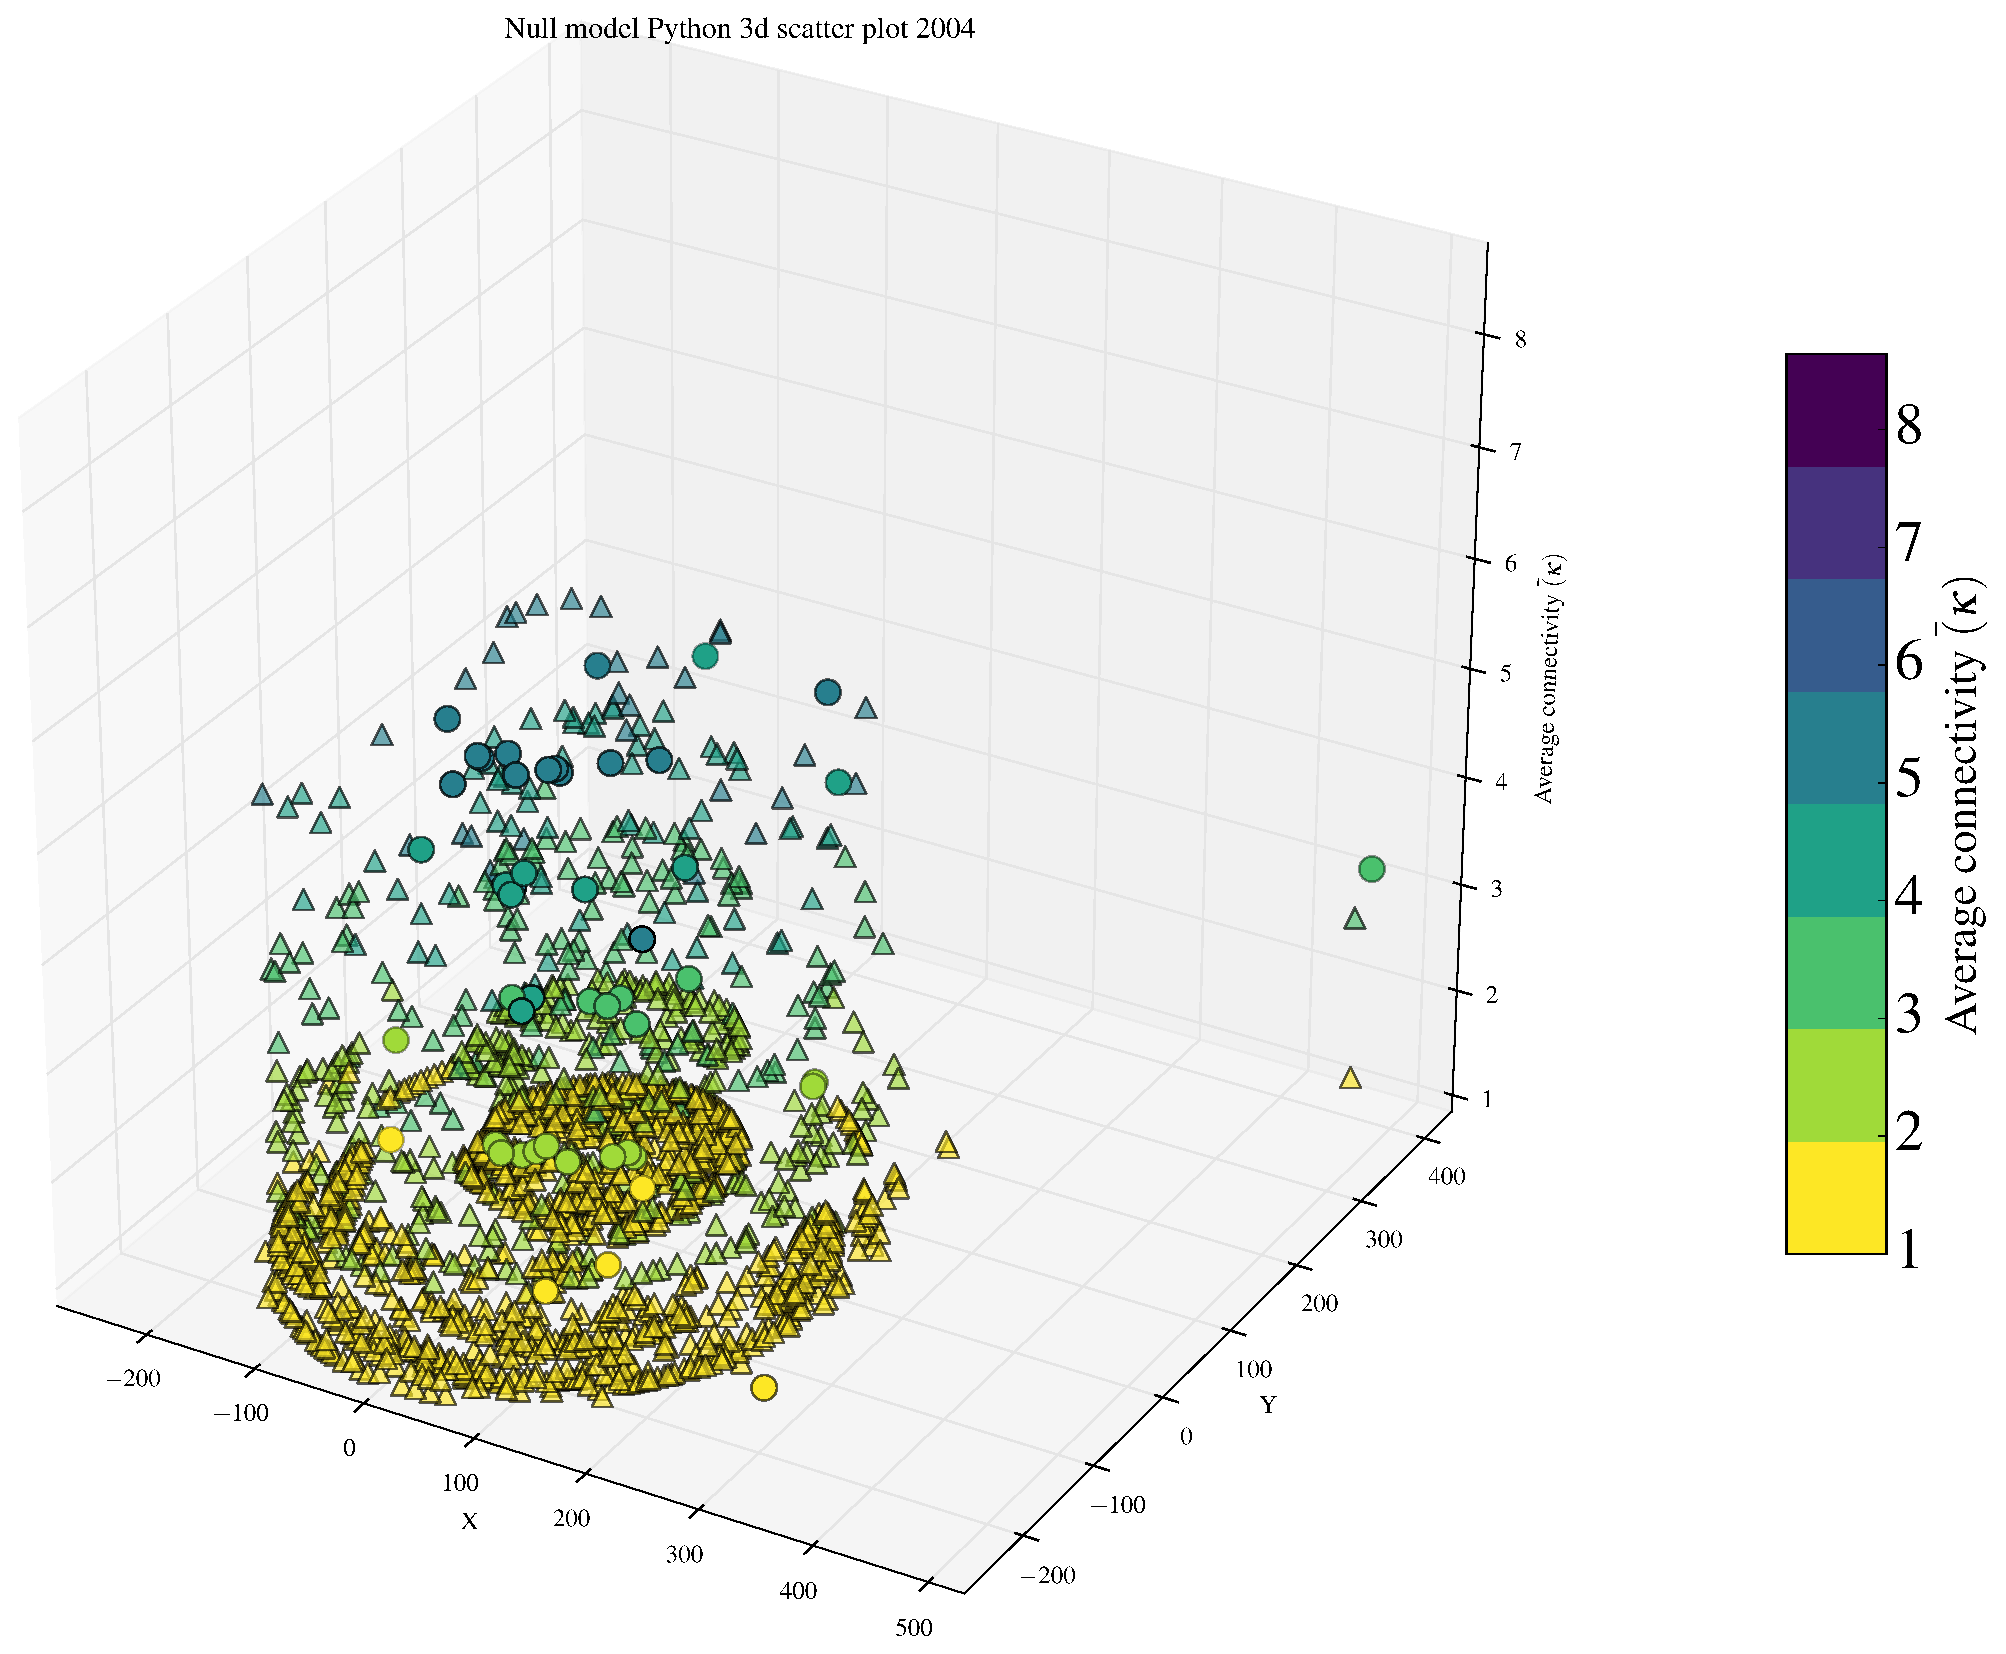
\includegraphics[scale=0.12]{../../figures/3d_scatter_python_2004_null}
\end{center}
\end{column}
\end{columns}

\end{frame}

\subsection{Cohesive Small World Model}

\begin{frame}
\frametitle{The Cohesive Small World Model}

The cooperation networks of both Debian and Python projects can be modeled using the proposed Cohesive Small World model.


\begin{columns}[c]
\begin{column}{0.5\textwidth}
\begin{block}{Small World Model}
\begin{itemize}
\item Fosters the flow of information through short paths.
\item Dense local clusters connected between them by relative short paths allow successful cooperation among heterogeneous individuals with common interests.
\end{itemize}
\end{block}
\end{column}

\begin{column}{0.5\textwidth}

\begin{block}{Structural Cohesion Model}
\begin{itemize}
\item Fosters trust and congruent values.
\item Individuals embedded in cohesive groups can compare independent perspectives on other members through a variety of relations that flow through distinct intermediaries.
\item Prevents the local clusters to be trapped in echo chambers of like minded       collaborators.
\end{itemize}
\end{block}
\end{column}
\end{columns}

\vspace{0.2cm}
But there are significative differences between Debian and Python.

\begin{columns}[c]
\begin{column}{0.5\textwidth}
\begin{block}{Debian Cooperation Networks}
\begin{itemize}
\item Lean more towards the Small World Model.
\item Subgroups work more independently from each other.
\item High modularity.
\end{itemize}
\end{block}
\end{column}

\begin{column}{0.5\textwidth}

\begin{block}{Python Cooperation Networks}
\begin{itemize}
\item Lean more towards the Structural Cohesion Model. 
\item Sharper and steep connectivity hierarchy.
\item Less modularity.
\end{itemize}
\end{block}
\end{column}
\end{columns}

\end{frame}


\section{Connectivity Hierarchy and Individual Contributions}

\begin{frame}
\frametitle{Dynamic Hierarchies as Open Elites}

The analysis of the hierarchical structure of organizations has been a central topic on organizational research in the last decades.

\begin{block}{Dynamic Analysis of Hierarchies}
Focus the analysis on the ratio of renewal of the individuals in the positions defined by that hierarchy.

\begin{description}
\item[Open Elite] ``reconceptualization of the concept of elite, more as a fluidly reproduced ideal than as a stable demographic reality'' \citep[360]{padgett:2010}.
\end{description}

\end{block}

\vspace{0.5cm}

I propose that hierarchical structures can be classified in a continuum, the two extreme points of which are: 

\begin{description}
\item[Static Hierarchy] where when an individual is appointed in a position of the hierarchy, this position is for life.
\item[Dynamic Hierarchy] where the individuals occupying positions defined by the hierarchy have a very high pace of renewal.
\end{description}

\end{frame}


\begin{frame}
\frametitle{The Hierarchical Structure of FOSS projects}

Free and Open Source Software (FOSS) communities have attracted a lot of attention from researchers. Academic efforts took mainly two directions:

\begin{columns}[c]
\begin{column}{0.5\textwidth}
\begin{block}{Reconcile with neoclassical economy}
\begin{itemize}
\item Mainly focused on the individual motivations of the participants. What is usually referred as ``microfundaments''.
\item Trying to explain motivations in terms of of rational self-interested individuals to match the dominant economic accounts.
\item Proposed that individuals 
\end{itemize}
\end{block}
\end{column}

\begin{column}{0.5\textwidth}

\begin{block}{Uncritically celebratory and a bit naive}
\begin{itemize}
\item Very influenced by practitioners account of the phenomenon.
\item Supported the ethical stand that valued more cooperation and reciprocity than competition and self-interest.
\item Assumed that FOSS communities are composed by loosely organized individuals with a very flat or nonexistent hierarchy among them.
\end{itemize}
\end{block}
\end{column}
\end{columns}

%\vspace{0.5cm}

\begin{block}{Well established empirical fact about FOSS projects}
\begin{itemize}
\item Only few of the participants account for the lion's share of the work done.
\item The deep contribution inequalities may mean that these projects follow the ``iron law of the oligarchy'' \citep{shaw:2014}.
\item I propose that one of the central characteristics of FOSS projects is their high ratio of turnover in key hierarchical positions.
\end{itemize}
\end{block}

\end{frame}


\begin{frame}
\frametitle{Empirical Analysis of Individual Contributions}

\note{The informal structure emerging from the patterns of cooperation among individuals in a FOSS project is quite hierarchical because reflects the fact that only few individuals are responsible for most contributions to the project.}

\begin{block}{Longitudinal Analysis of the Social Structure of FOSS projects}
The social structure of a community are the patterns of relations established among individual participants in the production process. But I do not limit the analysis to one point in time; I analyze its evolution.
\end{block}

\begin{columns}[c]
\begin{column}{0.5\textwidth}
\begin{block}{Puzzle: FOSS projects as Oligarchies?}
\citet{michels:1915} ``iron law of oligarchy'' states that organizations tend towards oligarchy as they grow, even if democracy and participation are part of their core goals.
\end{block}
\end{column}

\begin{column}{0.5\textwidth}
\begin{block}{FOSS projects as Open Elites}
The continuous renewal of the people that does most of the work is a key mechanism to explain how FOSS projects can thrive and success through time.
\end{block}
\end{column}
\end{columns}

\vspace{0.2cm}

Results of the empirical analysis:

\begin{itemize}
\item The developers that contribute the most to the projects analyzed are in the higher levels of the connectivity structure of the project's cooperation networks. The hierarchical connectivity structure shapes the volume of contribution of individual developers.

\item My analysis shows that the ratio of renewal of individuals at these structural positions is quite fast, which characterizes FOSS communities as dynamic hierarchies and open
elites.

\item I found that the position of an individual in the connectivity structure of the cooperation network also impacts significantly in the median active life of a developer in the project.
\end{itemize}

\note{Thus, if we analyze cross-sectionally (ie in a concrete point of time) a FOSS project, a very small fraction of the participants are the ones that actually do the lion's share of contributions, as previous empirical research has shown. However if we analyze the evolution of contributions longitudinally, we find that the persons that contribute the most change through time.}

\end{frame}


\begin{frame}
\frametitle{Individual contributions by connectivity level}

\begin{figure}
\vspace{-0.6cm}
\centering
\subfloat[Debian: developer \% by connectivity level]{
\label{}
\includegraphics[scale=0.19]{../../figures/evolution_developers_debian_years}
}
\hspace{0.5cm}
\subfloat[Python: developer \% by connectivity level]{
\label{}
\includegraphics[scale=0.19]{../../figures/evolution_developers_python_years}
}
\hspace{0.1cm}
\subfloat[Debian: contributions by connectivity level]{
\label{}
\includegraphics[scale=0.19]{../../figures/evolution_connectivity_debian_years}
}
\hspace{0.5cm}
\subfloat[Python: contributions by connectivity level]{
\label{}
\includegraphics[scale=0.19]{../../figures/evolution_connectivity_python_years}
}
\label{fig:contributions}
\caption[]{}
\end{figure}

\end{frame}


\begin{frame}
\frametitle{Analyzing Source Code Contributions and beyond}
\note{From the figures on the previous slide, it is clear that there is a strong correlation between the connectivity level of a developer and her level of contribution to the project.

The hierarchical structure of the cooperation network shapes the volume of contribution of individual developers.}

To further the analysis I used more sophisticated statistical modeling strategies to assess the impact of the connectivity structure in the individual contributions to the project.

\begin{itemize}

\item \textbf{Debian package uploads:} Modeled with a negative binomial regression. Over-dispersed and discrete dependent variable: \# of uploads. The $k$-component number is the second most important independent variable only after Degree Centrality.

\item \textbf{Added source code lines to Python:} Modeled with a panel regression with individual and year fixed effect. Dependent variable treated as a continuous variable. The $k$-component number is also the second most important independent variable only after Degree Centrality.

\end{itemize}

\begin{block}{Potential endogenity problems of the previous models}
There is a relation between the dependent variable and the network metrics (independent variables) because the cooperation networks are build precisely based on contributions to the projects.
\end{block}

\begin{itemize}

\item \textbf{Number of accepted \textit{Python Enhancement Proposals} (PEP):} Modeled with a zero inflated negative binomial. PEPs are design documents that define the language; are thus contributions not directly related to the cooperation networks. Being part of the top connectivity level is also the second most important independent variable, this time only after developer's tenure (in years).

\end{itemize}


\end{frame}


\begin{frame}
\frametitle{Cooperation Networks' Connectivity Hierarchies as Open Elites}

\begin{figure}
\centering
\vspace{-0.2cm}
\hspace{-0.8cm}
\includegraphics[scale=0.22]{../../figures/sankey_mobility_python_years}
\caption{Sankey diagram of Python developer mobility at the top connectivity level.}
\end{figure}

\end{frame}

\begin{frame}
\frametitle{Cooperation Networks' Connectivity Hierarchies as Open Elites}

\begin{table}[h]
\caption{Developer mobility in the top connectivity level for the Python project.}
\label{python_mobility_table}
\begin{center}
\begin{tabular}{ccccc}
\toprule
Years&Top Developers&New Developers&Developers Out&Developers back \\ 
\midrule
1999&3 (33.3\%)&3 (100.0\%)&0 (0.0\%)&0 (0.0\%) \\ 
2000&11 (35.5\%)&8 (72.7\%)&1 (9.1\%)&0 (0.0\%) \\ 
2001&13 (39.4\%)&4 (30.8\%)&1 (7.7\%)&0 (0.0\%) \\ 
2002&19 (50.0\%)&8 (42.1\%)&1 (5.3\%)&0 (0.0\%) \\ 
2003&19 (45.2\%)&3 (15.8\%)&5 (26.3\%)&0 (0.0\%) \\ 
2004&14 (28.6\%)&3 (21.4\%)&1 (7.1\%)&0 (0.0\%) \\ 
2005&19 (43.2\%)&1 (5.3\%)&4 (21.1\%)&5 (26.3\%) \\ 
2006&12 (23.1\%)&0 (0.0\%)&4 (33.3\%)&1 (8.3\%) \\ 
2007&20 (39.2\%)&10 (50.0\%)&7 (35.0\%)&3 (15.0\%) \\ 
2008&21 (35.6\%)&6 (28.6\%)&6 (28.6\%)&3 (14.3\%) \\ 
2009&22 (37.9\%)&9 (40.9\%)&3 (13.6\%)&1 (4.5\%) \\ 
2010&28 (44.4\%)&9 (32.1\%)&7 (25.0\%)&2 (7.1\%) \\ 
2011&25 (39.7\%)&7 (28.0\%)&2 (8.0\%)&1 (4.0\%) \\ 
2012&32 (49.2\%)&8 (25.0\%)&12 (37.5\%)&4 (12.5\%) \\ 
2013&33 (52.4\%)&8 (24.2\%)&16 (48.5\%)&5 (15.2\%) \\ 
2014&20 (32.3\%)&3 (15.0\%)&0 (0.0\%)&0 (0.0\%) \\ 
\bottomrule
\end{tabular}
\end{center}
\end{table}

\end{frame}



\begin{frame}
\frametitle{Modeling robustness as median active live of individuals in the project}

\begin{figure}
\centering
\subfloat[Survival Function for all developers]{
\label{fig:survival_all}
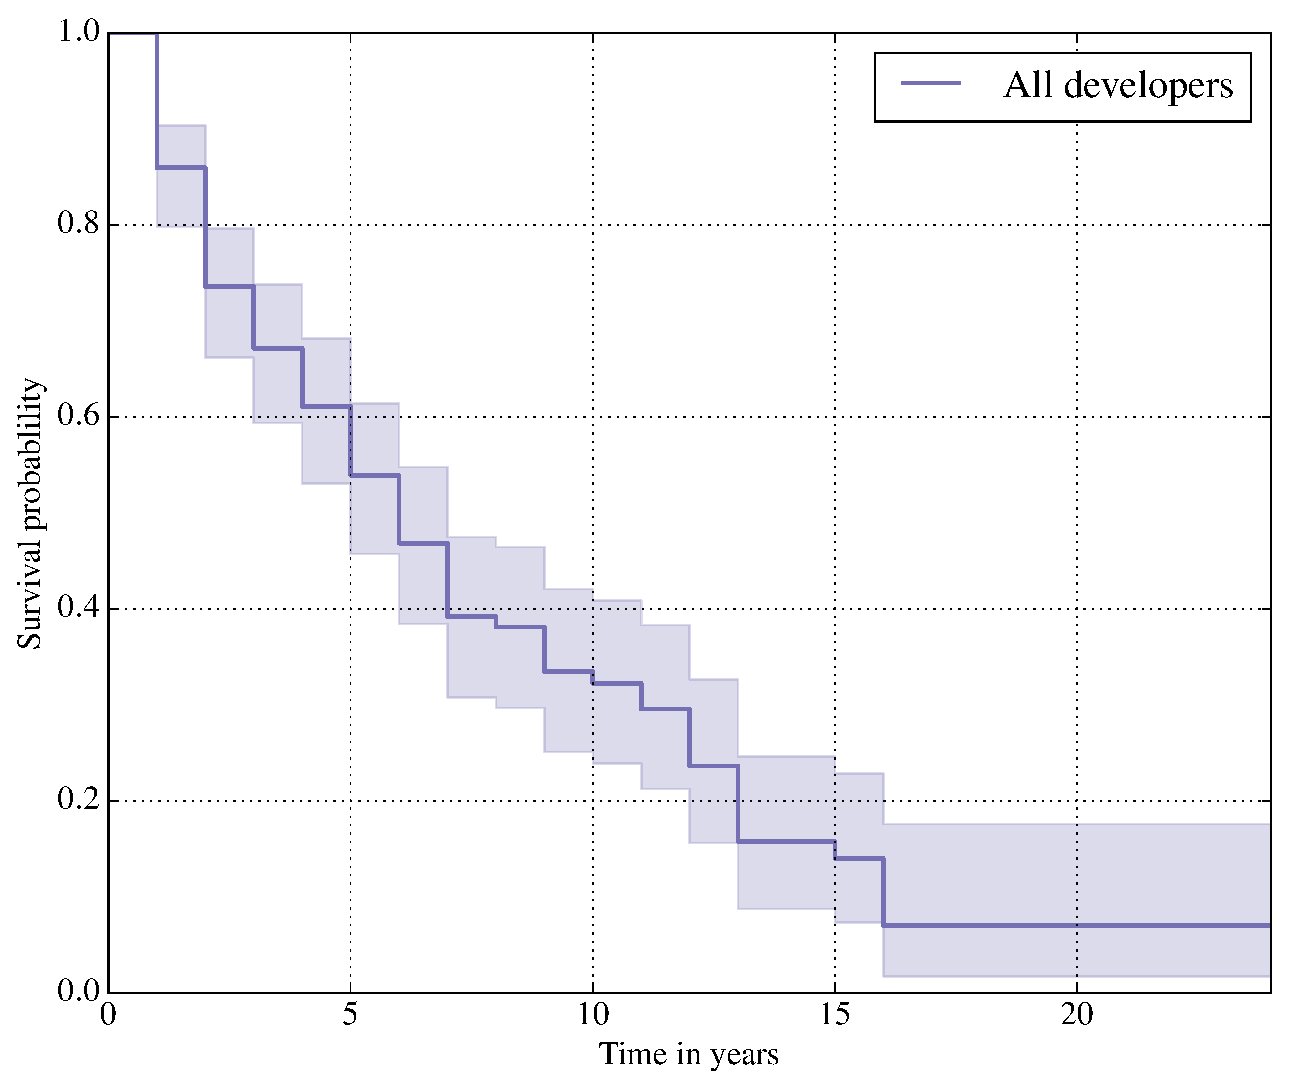
\includegraphics[scale=0.2]{../../figures/survival_all}
}
\hspace{.01in}
\subfloat[Survival Function for developers in the top connectivity level]{
\label{fig:survival_groups}
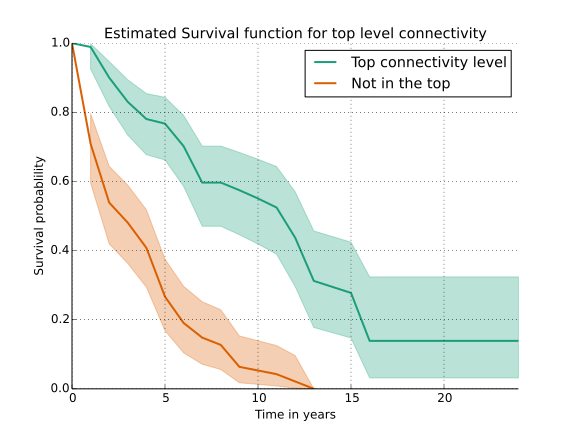
\includegraphics[scale=0.2]{../../figures/survival_top}
}
\label{fig:survival}
\caption[Survival function using the Kaplan-Meier estimate.]{Estimation of the survival function using the Kaplan-Meier estimate. The median survival time of a developer in the community, defined as the point in time where on average half of the population has abandoned the community, is 6 years if I consider all developers (left). But if I consider separately the developers in the top level of the connectivity hierarchy (right), their median survival time is 12 years; but only 3 years for the developers that are not on the top of the connectivity hierarchy.}
\end{figure}

\end{frame}

%\section{References}

\begin{frame}
\frametitle{Conclusions}

\begin{itemize}

\item \textbf{Cooperation Networks:} A meso level approach to large scale cooperation focused on the patterns of relations that direct producers establish between them in knowledge intensive production processes.

\item \textbf{The Cohesive Small World model}: The structural patterns defined by this model provide the scaffolding for enabling effective large scale cooperation.

\begin{itemize}
\item Structurally cohesive groups nested inside each other that form a connectivity hierarchy.

\item Dense local clusters connected between them by relative short paths.
\end{itemize}

\item I \textbf{developed heuristics} to compute the $k$-components structure that allow for the computing of the approximate value of group cohesion for moderately large networks in a reasonable time frame. I \textbf{contributed an implementation} of these heuristics to a popular Python software package for the analysis of complex networks: NetworkX \citep{hagberg:2008}.

\item The ``Cohesive Small World'' model is a good fit to describe the cooperation networks ---that is, the patterns of relations between direct producers--- of two big and mature FOSS projects: the Python programming language, and the Debian operating system.

\item The nested structure of $k$-components nicely captures the hierarchy in the patterns of relations that individual contributors establish when working together. This hierarchy:

\begin{itemize}
\item reflects the empirically well established fact that in FOSS projects only a small fraction of the developers account for most of the contributions.

\item refutes the naive views of early academic accounts that characterized FOSS projects as a flat hierarchy of peers in which every individual does more or less the same.
\end{itemize}

\item \textbf{Cooperation has a structural dimension} because membership in cohesive groups that emerge from the cooperation networks has an important and statistically significative impact on both the volume of individual contributions, and on the median active life of developers.

\item The connectivity structure of collaborative communities' cooperation networks can be characterized as an \textbf{open elite}, where the top levels of this hierarchy are filled with new individuals at a high pace. This feature is key for understanding the mechanisms and dynamics that make FOSS communities able to develop long term projects, with high individual turnover, and yet achieve high impact and coherent results as a result of large scale cooperation.

\item However, it is not clear that the theoretical model that I proposed fits all cooperation networks of Collaborative Communities, or even cooperation networks of all FOSS projects. Because the empirical analysis presented in this thesis was a case study of two successful projects aimed to develop a theoretical framework, I cannot determine if other FOSS projects also fit nicely in it. Thus what I presented is more an existence proof than a empirical test of my proposed theoretical model.

\end{itemize}

\note{
\begin{itemize}
\item The generation of trust and congruent values among heterogeneous individuals are fostered by structurally cohesive groups in the connectivity hierarchy of cooperation networks because individuals embedded in these structures are able to compare independent perspectives on each other through a variety of paths that flow through distinct sets of intermediaries, which provides multiple independent sources of information about each other. This mediated perception of the group generates trust at a global scale.

\item The existence of dense local clusters connected between them by relative short paths allows successful cooperation among heterogeneous individuals with common interests and, at the same time, fosters the flow of information between these clusters preventing the local clusters to be trapped in echo chambers of like minded collaborators.
\end{itemize}
}

\end{frame}


\begin{frame}[label=biblio]
\frametitle{References}
% Bibliografia
\begin{tiny}
\bibliographystyle{chicago}
\bibliography{../../thesis.bib}
\end{tiny}
\end{frame}

\end{document}
